\documentclass[12pt, letterpaper, preprint]{aastex}
\usepackage[breaklinks,colorlinks, urlcolor=blue,citecolor=blue,linkcolor=blue]{hyperref}
\usepackage{color}
\usepackage{amsmath}
\usepackage{natbib}
\usepackage{ctable}
\usepackage{bm}
%%% This file is generated by the Makefile.
\newcommand{\giturl}{\url{https://github.com/changhoonhahn/nonGaussLike}}
\newcommand{\githash}{0cff07b}\newcommand{\gitdate}{2018-01-09}\newcommand{\gitauthor}{ChangHoon Hahn}


% typesetting shih
\linespread{1.08} % close to 10/13 spacing
\setlength{\parindent}{1.08\baselineskip} % Bringhurst
\setlength{\parskip}{0ex}
\let\oldbibliography\thebibliography % killin' me.
\renewcommand{\thebibliography}[1]{%
  \oldbibliography{#1}%
  \setlength{\itemsep}{0pt}%
  \setlength{\parsep}{0pt}%
  \setlength{\parskip}{0pt}%
  \setlength{\bibsep}{0ex}
  \raggedright
}
\setlength{\footnotesep}{0ex} % seriously?

% citation alias
\defcitealias{beutler2017}{B2017}
\defcitealias{sinha2017a}{S2017}

% math shih
\newcommand{\setof}[1]{\left\{{#1}\right\}}
\newcommand{\given}{\,|\,}
\newcommand{\pseudo}{{\mathrm{pseudo}}}
\newcommand{\Var}{\mathrm{Var}}

\newcommand{\specialcell}[2][c]{%
  \begin{tabular}[#1]{@{}c@{}}#2\end{tabular}}
% text shih
\newcommand{\foreign}[1]{\textsl{#1}}
\newcommand{\etal}{\foreign{et~al.}}
\newcommand{\opcit}{\foreign{Op.~cit.}}
\newcommand{\documentname}{\textsl{Article}}
\newcommand{\equationname}{equation}
\newcommand{\bitem}{\begin{itemize}}
\newcommand{\eitem}{\end{itemize}}
\newcommand{\beq}{\begin{equation}}
\newcommand{\eeq}{\end{equation}}
\newcommand{\todo}[1]{{\bf \textcolor{red}{#1}}}
\newcommand{\Dmock}{\mathbf{D}^\mathrm{mock}}
\newcommand{\Xmock}{{\bf X}^\mathrm{mock}}
\newcommand{\Xref}{{\bf X}^\mathrm{ref}}
\newcommand{\Yref}{{\bf Y}^\mathrm{ref}}
\newcommand{\Ralpha}{R\'enyi-$\alpha$}
\newcommand{\Beut}{\citetalias{beutler2017}}
\newcommand{\Sinh}{\citetalias{sinha2017a}}

\newcommand{\patchy}{{\fontshape\scdefault\selectfont patchy}}

\begin{document}\sloppy\sloppypar\frenchspacing 

%\title{How I Learned to Stop Worrying and Love The Central Limit Theorem}
\title{Likelihood Non-Gaussianity in Large Scale Structure Analyses}
\date{\texttt{DRAFT~---~\githash~---~\gitdate~---~NOT READY FOR DISTRIBUTION}}
\author{ChangHoon~Hahn\refstepcounter{footnote}\refstepcounter{footnote}, et al.} %Florian~Beutler, Manodeep~Sinha, Andreas~Berlind}
\affil{Lawrence Berkeley National Laboratory, 1 Cyclotron Rd, Berkeley CA 94720, USA}
\email{changhoon.hahn@lbl.gov}

\begin{abstract}
    Standard present day large-scale structure (LSS) analyses make a major 
    assumption in their Bayesian parameter inference --- the likelihood has 
    a Gaussian functional-form. We investigate the impact of this assumption 
    on two recent LSS analyses: the \cite{beutler2017}~powerspectrum multipole ($P_\ell$) analysis and 
    the \cite{sinha2017a}~group multiplicity function ($\zeta$) analysis. Using non-parametric 
    divergence estimators on mock catalogs originally constructed for covariance matrix 
    estimation in these analyses, we identify significant non-Gaussianity for both 
    $P_\ell$ and $\zeta$ 
    %quantify the non-Gaussianity of the $P_\ell$ and $\zeta$ likelihoods. We 
    likelihoods. Afterwards, we use Gaussian mixture density estimation and 
    Independent Component Analysis to construct likelihood estimates that better 
    approximate the true likelihood than the Gaussian \emph{pseudo}-likelihood. 
    We then use the likelihood estimates to derive the true posterior probability 
    distribution of the \Beut~and~\Sinh~parameters. Our parameter constraints reveal 
    the impact of likelihood non-Gaussianity on the posterior parameter constraints 
    of \Beut~and~\Sinh. Despite some impact on the $f\sigma_8$ constraint, 
    likelihood non-Gaussianity does not significantly impact the overall 
    \Beut~parameter constraints. For the $\zeta$ analysis, 
    however, using the pseudo-likelihood significantly underestimates the 
    uncertainties and biases the constraints of \Sinh~halo occupation parameters: 
    $\log\,M_\mathrm{min}$, $\log\,M_1$ and $\alpha$. The divergence and 
    likelihood estimation methods we present provides a straightforward framework
    for quantifying the impact of likelihood non-Gaussianity and deriving more 
    accurate parameter constraints. 
\end{abstract}

\keywords{
methods: statistical
---
galaxies: statistics
---
methods: data analysis
---
cosmology: observations
---
cosmological parameters
---
large-scale structure of universe
}

\section{Introduction}


\begin{itemize}
    \item Talk about the use of Bayesian parameter inference and getting the posterior in LSS cosmology 
    \item Explain the two major assumptions that go into evaluating the likelihood
    \item Emphasize that we are not talking about non-Gaussian contributions to the likelihood
    \item Emphasize the scope of this paper is to address whether one of the assumptions matters for 
        galaxy clustering analyses. 
\end{itemize}

The motivation for the Gaussian pseudo-likelihood ultimately stems 
from the Central Limit Theorem. The powerspectrum of the density field, 
for instance, is the correlation function of the density field. Assuming 
that the density field is a Gaussian random field, which it approximately 
is, the powerspectrum of a specific mode would follow a chi-squared 
distribution. With sufficiently many independent modes contributing, 
from Central Limit Theorem, the likelihood of the powerspectrum would 
\emph{approach} a Gaussian distribution. In practice, due to finite 
survey volume, shot noise, and systematic effects different modes
are correlated and the Gaussian likelihood assumption cannot be true 
for the powerspectrum. In low signal-to-noise regimes we explicitly 
expect the Gaussian assumption to fail. \cite{scoccimarro2000} 
\todo{provides an excellent example of how the Gaussianity 
illustrates how the }
this for the powerspectrum. 
%At scales where non-linear effects become important, k ≈ 0.2 − 0.3 h/Mpc, the density field cannot be assumed to be Gaussian anymore. A complementary approach at these scales is to consider that the power spectrum distribution about its mean is Gaussian; if there are enough independent modes contributing to a given shell in Fourier space, by the central limit theorem the distribution of the power spectrum should approach Gaussianity. However, due to the finite volume of the survey and shot noise, different modes are correlated, so it is not clear a priori at what scales Gaussianity applies. 

\todo{talk about CMB likelihood analyses? Bring up sellentin et al.'s t-distribution stuff?}
Hence for precise parameter constraints, LSS analyses using the Gaussian 
pseudo-likelihood must insure that their analysis is conducted in sufficiently high 
signal-to-noise regimes and test the impact of likelihood non-Gaussianity. 
This is unfortunately not a part of the standard practice in LSS studies. 

% Data analysis can only lead to unbiased constraints on a physical theory if the employed likelihood is correct (e.g.  Trotta 2008; Mardia et al. 1979; Anderson 2003; Cramer 1946; Jeffreys 1961; Sun & Berger 2006). 

In this paper we investigate the impact of the likelihood Gaussianity
assumption on the two recent LSS analyses of \cite{beutler2017} (hereafter~\Beut)
and \cite{sinha2017a} (hereafter~\Sinh). \Beut~analyzes the powerspectrum 
multipoles ($P_\ell$; monopole, quadrupole, and hexadecapole) to measure
redshift-space distortions along with the Alcock–Paczynski effect and baryon 
acoustic oscillation scale. Meanwhile \Sinh~analyzes the group multiplicity 
function ($\zeta$) in order constrain parameters of the halo model.
Using the~\Beut~and~\Sinh~analyses, we show in this paper that the assumption 
of likelihood Gaussianity in LSS is not necessary. We will also show that 
the mock catalogs used in standard LSS analyses for covariance matrix estimation 
can be used to quantify the non-Gaussianity. More importantly the mocks can be 
used to estimate the ``true'' non-Gaussian likelihood. 

We begin in Section~\ref{sec:mocks} by describing the mock catalogs, 
which we use throughout the paper, constructed originally for covariance 
matrix estimation in~\Beut~and~\Sinh. Next in Section~\ref{sec:div}, we present
non-parametric divergence estimators and quantify the non-Gaussianity of
the $P_\ell$ and $\zeta$ likelihoods using them. Then in Section~\ref{sec:likeest}, 
we introduce two methods for estimating the ``true'' likelihood using the 
mock catalogs. We then use the likelihood estimates to quantify the impact 
of likelihood non-Gaussianity on the posterior parameter constraints 
of~\Beut~and~\Sinh. We discuss and conclude the paper in Section~\ref{sec:summary}.  

\section{Mock Catalogs} \label{sec:mocks}
Mock catalogs play an indispensable role in standard cosmological 
anslyses of LSS studies. They're used for testing analysis 
pipelines~\citep[][]{beutler2017, grieb2017, tinkerinpreparation}, 
testing the effect of systematics~\citep{guo2012, vargas-magana2014, hahn2017, pinol2017, ross2017}, 
and, most relevantly for this paper, estimating the covariance 
matrix~\citep[][]{parkinson2012, kazin2014, grieb2017, alam2017, beutler2017, sinha2017a}. 
In fact, nearly all current state-of-the-art LSS analyses use
covariance matrices estimated from mocks to evaluate the likelihood 
for parameter inference. 

While some argue for analytic estimates of the covariance 
matrix~\citep[e.g.][]{mohammed2017} or estimates directly from data
by subsampling~\citep[e.g.][]{norberg2009}, covariance matrices 
from mocks have a number of advantages. Mocks allow us 
to incorporate detailed systematic errors present in the 
data and variance beyond the volume of the data. Even for analytic 
estimates, a large ensemble of mocks are crucial for validation~\citep[\emph{e.g.}][]{slepian2017}. 
Moreover, as we show later in this paper, mocks present an
additional advantage: they allow us to 
quantify the non-Gaussianity of the likelihood and more accurately 
estimate the true likelihood distribution. 

In this paper, we focus on two LSS analyses: the powerspectrum 
multipole ($P_\ell$) analysis of \Beut~and group multiplicity 
function ($\zeta$) analysis of \Sinh. Throughout the paper we will 
make extensive use of the mock catalogs used in these analyses. 
In this section, we give a brief description of these mocks and how 
the observables used in the analysis --- the powerspectrum 
multipole ($P_\ell$) and group multiplicity function ($\zeta$) ---
are calculated from them. Afterwards, we will describe how we compute 
the covariance matrix from the mocks and pre-process the mock observable
data.

\subsection{MultiDark-PATCHY~Mock Catalog} \label{sec:patchy}
In their powerspectrum multipole analysis, \Beut~use 
the MultiDark-\patchy~mock catalogs from \cite{kitaura2016}. 
These mocks are generated using the \patchy~code \citep{kitaura2014,kitaura2015}. 
They rely on large-scale density fields generated using augmented
Lagrangian Perturbation Theory~\citep[ALPT;][]{kitaura2013} on a mesh,
which they then populate with galaxies based on a combined non-linear
deterministic and stochastic biases. The mocks from the \patchy~code 
are then calibrated to reproduce the galaxy clustering in the 
high-fidelity BigMultiDark $N$-body simulation~\citep{rodriguez-torres2016, klypin2016}. 
Afterwards, the galaxies are assigned stellar masses using the 
{\fontshape\scdefault\selectfont hadron}~code~\citep{zhao2015}.
and the {\fontshape\scdefault\selectfont sugar}~code~\citep{rodriguez-torres2016} 
is applied to combine different boxes, incorporate selection
effects and masking to produce mock light-cone galaxy catalogs. 
The statistics of the resulting mocks are then compared to 
observations and the process is iterated to reach desired 
accuracy. We refer readers to~\cite{kitaura2016} for further 
details. 

In total, \cite{kitaura2016} generated 12,228 mock light-cone 
galaxy catalogs for BOSS Data Release 12. In \Beut, 
they use 2045 and 2048 for the northern galactic cap (NGC) and 
southern galactic cap (SGC) of the LOWZ+CMASS combined sample. 
\Beut~excluded 3 mock realizations due to notable 
issues. These issues have since been addressed so in our analysis 
we use all 2048 mocks for both the NGC and SGC of the LOWZ+CMASS
combined sample. In \Beut, they conduct multiple analyses, 
some using only the powerspectrum monopole and quadrupole 
and others using monopole, quadrupole, and hexadecapole. They 
also separately analyze three redshift bins: $0.2 < z < 0.5$, 
$0.4 < z < 0.6$, and $0.5 < z < 0.75$. In this paper we focus on 
one of these analyses: the analysis of the powerspectrum monopole, 
quadrupole, and hexadecapole for the $0.2 < z < 0.5$ bin.  

\subsection{\cite{sinha2017a} Mocks} \label{sec:gmf} 
The simulations used in the small-scale clustering analysis of \cite{sinha2017a} 
are from the Large Suite of Dark Matter Simulations project~\citep[LasDamas;][]{mcbride2009} 
designed to model galaxy samples from SDSS DR7. They use initial conditions derived from 
second order Lagrangian Perturbation Theory using the 2LTPIC code~\citep{scoccimarro1998, crocce2006}
and evolved them using the $N$-body $\mathtt{GADGET}$-$2$ code~\citep{springel2005}.
Halos are then identified from the dark matter distribution outputs using 
the $\mathtt{ntropy-fofsv}$ code~\citep{gardner2007}, which uses a 
friend-of-friends algorithm~\citep[FoF;][]{davis1985} with a linking length of $0.2$
times the mean inter-particle separation. %The FoF halo masses are then adjusted using the \cite{warren2006} correction. 
\Sinh~uses two configurations of the LasDamas simulations for the 
$M_r < -19$ and $M_r < -21$ samples of SDSS DR7.
The Consuelo simulation contains $1400^3$ dark matter particles with 
mass of $1.87 \times 10^9\,h^{-1} M_\odot$ in a cubic volume of 
$420\,h^{-1} Mpc$ per side evolved from $z_\mathrm{init} = 99$. 
The Carmen simulation contains $1120^3$ dark matter particles with mass 
of $4.938 \times 10^{10}\,h^{-1} M_\odot$ in a cubic volume of 
$1000\,h^{-1} Mpc$ per side evolved from $z_\mathrm{init} = 49$. 
%They use the following cosmological parameters, which are motivated by the WMAP3 constraints \citep{spergel2007}: $\Omega_m = 0.25, \Omega_\Lambda = 0.75, \Omega_b = 0.04, h = 0.7, \sigma_8 = 0.8,\;\mathrm{and}\;n_s = 1.0.$

The FoF halo catalogs are then populated with galaxies using the 
`Halo Occupation Distribution` (HOD) framework. The 
number, positions, and velocities of galaxies are described statistically 
by an HOD model. \Sinh~adopts the `vanilla' HOD model of \cite{zheng2007}, 
where the mean number of central and satellite galaxies are described by 
the halo mass and five HOD parameters: $M_\mathrm{min}, 
\sigma_{\log\,M} , M_0, M_1,~\mathrm{and}~\alpha$. Lastly, once the 
simulation boxes are populated with galaxies, observational systematic 
effects are imposed. The peculiar velocities of galaxies are used to 
impose redshift-space distortions. Galaxies that lie outside the redshift
limits or sky footprint of the SDSS sample are removed. For further 
details regarding the mocks, we refer readers to \Sinh.

To calculate their covariance matrix, \Sinh~produced 200 
independent mock catalogs from 50 simulations using a single set of 
HOD model parameters. To take advantage of the methods we later 
present, we require a large 
number of mocks. Our methods rely on using the mocks to sample high 
dimensional distributions, so incorporating more mocks improves their 
accuracy. We utilize an addition $99$ sets of HOD parameters with $200$
mocks each. These parameters are sampled from the MCMC chain used to 
produce the posterior in~\Sinh. In total we use $20,000$ mocks. 
Among the multiple analyses in \Sinh, in this paper we focus on the 
GMF analysis of the SDSS DR7 $M_r < -19$ sample. 

\subsection{Mock Observable ${\bf X}^\mathrm{mock}$ and Covariance Matrix $\mathbb{C}$} \label{sec:xmock}
To get from the mock catalogs described above to the covariance matrices 
used in~\Beut~and~\Sinh, the observables are measured for each mock in 
the \emph{same} way as the observations. We briefly describe how $P_\ell(k)$ and $\zeta(N)$ 
and their covariance matrices are measured in \Beut~and \Sinh. We then 
describe how we pre-process the mock observables for the methods we describe 
in the next sections.

To measure the powerspectrum multipoles of the BOSS DR12 galaxies
and the MutliDark-\patchy~mocks (Section~\ref{sec:patchy}), \Beut~uses a 
fast Fourier transform (FFT) based anisotropic powerspectrum estimator 
based on \cite{bianchi2015} and \cite{scoccimarro2015}. This estimator 
estimates the  monopole, quadrupole, and hexadecapole 
($\ell = 0, 2,\,\mathrm{and}\,4$) of the powerspectrum using FFTs of the 
overdensity field multipoles for a given survey geometry. For further 
details on the estimator we refer readers to~\Beut~Section 3. \Beut~compute
the powerspectrum over the range $k = 0.01 - 0.15\, h\,\mathrm{Mpc}^{-1}$
for $\ell = 0,\,\mathrm{and}\,2$ and $k = 0.01 - 0.10\, h\,\mathrm{Mpc}^{-1}$.
for $\ell = 4$. The powerspectrum multipoles are calculated in bins of 
$\Delta k = 0.01\,h\,\mathrm{Mpc}^{-1}$.

From the $\vec{P}^{(n)} = \big[P^{(n)}_{0}(k), P^{(n)}_{2}(k), P^{(n)}_{4}(k) \big]$ 
of the MultiDark-\patchy~mocks, \Beut~computes the $(i, j)$ element of the 
covariance matrix of all multipoles as 
\beq
\mathbb{C}_{i,j} = \frac{1}{N_\mathrm{mock} - 1} \sum\limits_{n=1}^{N_\mathrm{mock}} \big[ \vec{P}^{(n)}_i - \overline{P}_i \big]
    \times \big[ \vec{P}^{(n)}_j - \overline{P}_j \big].
\eeq
$N_\mathrm{mock} = 2048$ is the number of mocks and $\overline{P}_i$ is the mean 
of the mock powerspectra: $\overline{P}_i = \frac{1}{N_\mathrm{mock}} \sum_{n=1}^{N_\mathrm{mock}} \vec{P}^{(n)}_i$.
Since $P_0$ and $P_2$ each have $14$ bins and $P_4$ has $9$ bins, 
$\mathbb{C}$ is a $37 \times 37$ matrix.
In this work, we compute the $P_\ell(k)$ using a similar FFT-based 
estimator of \cite{hand2017a} instead of the~\Beut~estimator. Our choice 
is based on computational convenience. A python implementation
of the \cite{hand2017a} estimator is publicly available in the $\mathtt{NBODYKIT}$ 
package\footnote{http://nbodykit.readthedocs.io/en/latest/index.html}~\citep{hand2017b}. 
We confirm that the resulting $P_\ell(k)s$ and covariance matrices from 
the two estimators are consistent with one another. 

Next, for the \Sinh~group multiplicity function analysis, they start 
with the \cite{berlind2006} FoF algorithm to identify groups in the 
SDSS and mock data. \Sinh~adopts the \cite{berlind2006} linking lengths
in units of mean inter-galaxy separation: $b_\perp = 0.14$ and $b_\parallel = 0.75$.
In comoving lengths, the linking lengths for the SDSS DR7 $M_r < -19$ 
sample correspond to $(r_\perp, r_\parallel) = (0.57, 3.05)h^{-1}\,\mathrm{Mpc}$. 
Once the groups are identified in the SDSS and mock data, $\zeta(N)$
is derived by calculating the comoving number density of groups 
in bins of richness $N$ --- the number of galaxies in the group. 
For the $M_r < −19$ SDSS sample, \Sinh~uses eight $N$ bins: 
$(5 - 6), (7 - 9), (10 - 13), (14 - 19), (20 - 32), (33 - 52), (53 - 84), (85 - 220)$.
For further details on the GMF calculation, we refer readers to 
\Sinh~Section 4.2.  
From the $\zeta^{(n)}(N)s$ of each mock, \Sinh~computes the $(i, j)$ element of
the covariance matrix as 
\beq \label{eq:gmf_cov} 
\mathbb{C}_{i,j} = \frac{1}{N_\mathrm{mock} -1} \sum\limits_{n=1}^{N_\mathrm{mock}} \big[\zeta^{(n)}(N_i) -  \bar{\zeta}(N_i)\big] \times
    \big[\zeta^{(n)}(N_j) -  \bar{\zeta}(N_j)\big].
\eeq
In \Sinh, they compute the covariance matrix using $200$ mocks
generated using a single fiducial set of HOD parameters. As we 
describe in Section~\ref{sec:gmf}, in this paper we use $20,000$ mocks from 
$100$ different set of HOD parameters sampled from the MCMC chain. 
The GMF covariance matrix we use in this paper is computed with 
$N_\mathrm{mock} = 20,000$ mocks. 

For the rest of the paper, in order to discuss the two separate 
analyses of~\Beut~and~\Sinh~in a consistent manner, we define the matrix 
$\Dmock$ of the mock observables ($P_\ell$ and $\zeta$) as 
\beq
\Dmock = \Big\{{\bf D}^\mathrm{mock}_n \Big\} \quad\quad \mathrm{where}\,\,\Dmock_n
\begin{cases}
    \vec{P}^{(n)} &\quad\mathrm{for}\,\, \mathrm{B}2017,\\ 
    \zeta^{(n)} &\quad\mathrm{for}\,\, \mathrm{S}2017.
\end{cases} 
\eeq
$\Dmock$ has dimensions of $2048 \times 37$ and $20,000\times8$ 
for \Beut~and \Sinh~respectively. 

For the methods in Sections~\ref{sec:gmm}~and~\ref{sec:ica}, the mock 
observable data ($\Dmock$) need to be pre-processed. This pre-processing
involves two steps: mean-subtraction (centering) and whitening. For mean subtraction, 
the mean of the observable is subtracted from $\Dmock$. Then 
$\Dmock - \overline{\bf D}^\mathrm{mock}$ is whitened using a linear transformation 
to remove the Gaussian correlation between the bins of $\Dmock$: 
\beq
\Xmock = L\,(\Dmock - \bar{\bf D}^\mathrm{mock}). 
\eeq
The linear transformation is derived so that covariance matrix of the whitened 
data, $\Xmock$, is the identity matrix $\mathbb{I}$. Such a whitening linear 
transformation can be derived in infinite ways. 
One way to derive the linear transformation is through the eigen-decomposition
of the covariance matrix~\citep[\emph{e.g.}][]{hartlap2009, sellentin2017}. We, alternatively, 
derive the linear transformation ${\bf L}$ using Choletsky decomposition of the 
inverse covariance matrix~\citep{Press:1992:NRC:148286}: 
$\mathbb{C}^{-1} = {\bf L}\,{\bf L}^T$. The different methods for whitening 
do not impact the results of the paper. Now that we have the pre-processed 
data of the mock observables, we proceed in the next section to quantifying 
the non-Gaussianity of the $P_\ell$ and $\zeta$ likelihoods. 


\section{Quantifying the Likelihood non-Gaussianity} \label{sec:div}
The standard approach to parameter inference in LSS studies neglects
to account for likelihood non-Gaussianity. 
However, we are not the first to investigate likelihood non-Gaussianity 
in LSS analyses. Nearly two decades ago, \cite{scoccimarro2000} examined 
the likelihood non-Gaussianity for the powerspectrum and reduced bispectrum 
using mock catalogs of the IRAS redshift catalogs. More recently, 
\cite{hartlap2009} and \cite{sellentin2017} examined the non-Gaussianity 
of the cosmic shear correlation function likelihood using simulations of 
the Chandra Deep Field South and CFHTLenS, respectively. 

While these works present different methods for identifying 
likelihood non-Gaussianity, they do not present a concrete way of 
quantifying it. \cite{hartlap2009}, for instance, identifies the
non-Gaussianity of the cosmic shear likelihood by looking at the
statistical independence/dependence of PCA components of the mock 
observable. In \cite{sellentin2017}, they use the Mean
Integrated Squared Error (MISE) as a distance metric between 
Gaussian random variables and the whitened mock observable 
data vector to characterize non-Gaussian correlations between elements 
of the data vector. These indirect measures of non-Gaussianity 
are challenging to interpret and extend more generally to LSS studies. 
%Sellentin & Heavens (2018) presented stringent tests that characterize non-Gaussian statistical behaviour, and any sound weak lensing likelihood should hence pass these tests.  The methods derived in Sellentin & Heavens (2018) test whether all pairwise combinations of data elements display the correct statistical behaviour under addition, division and multiplication, and whether the correct marginal distribution ensues for each data point. 

A more direct approach, however, can be taken to quantify the 
non-Gaussianity of the likelihood. We can calculate the divergence between 
the distribution of our observable, $p(x)$, and $q(x)$ a multivariate Gaussian described 
by the average of the mocks and the covariance matrix.
The following are two of the most commonly used divergences: 
the Kullback-Leibler (KL) divergence
\beq \label{eq:kl} 
D_{KL} ( p \parallel q ) = \int p(x)\,\log \frac{p(x)}{q(x)}\,{\rm d}x
\eeq
and the R\'enyi-$\alpha$ divergence
\beq \label{eq:renyi}
D_{R-\alpha} ( p \parallel q ) = \frac{1}{\alpha -1} \log \int p^\alpha(x)\, q^{1 -\alpha}(x)\,{\rm d}x. 
\eeq
In the limit as $\alpha$ approaches 1, the R\'enyi-$\alpha$ divergence is
equivalent to the KL divergence.
%To evaluate the R\'enyi-$\alpha$ divergence, we need to evaluate the following
%kernel function
%\beq \label{eq:d_alpha}
%D_{\alpha} ( p \parallel q ) = \int p^\alpha(x) q^{1-\alpha}(x)\,{\rm d}x. 
%\eeq

Of course, in our case, we don't know $p(x)$ --- \emph{i.e.} the distribution of
our observable. If we did, we would simply use that instead of bothering with 
the covariance matrix or this paper. We can, however, still estimate the 
divergence using nonparametric divergence estimators~\citep{wang2009, poczos2012, krishnamurthy2014}. 
These estimators allow us to estimate the divergence directly from 
samples $X_{1:n} = \{ X_1, ... X_n \}$ and $Y_{1:m} = \{ Y_1, ... Y_m \}$ 
drawn from $p$ and $q$ respectively: $\hat{D}_{\alpha}(X_{1:n} \parallel Y_{1:m})$. 
For instance, the estimator presented in \cite{poczos2012} allows us to estimate 
the kernel function of the R\'enyi-$\alpha$ divergence,
\beq \label{eq:d_alpha}
D_{\alpha} ( p \parallel q ) = \int p^\alpha(x) q^{1-\alpha}(x)\,{\rm d}x. 
\eeq
using $k^\mathrm{th}$ nearest neighbor density estimators. Let $\rho_k(x)$ 
denote the Euclidean distance of the $k^\mathrm{th}$ nearest neighbor 
of $x$ in the sample $X_{1:n}$ and $\nu_k(x)$ denote the Euclidean distance 
of the $k^\mathrm{th}$ nearest neighbor of $x$ in the sample $Y_{1:m}$. Then 
\beq \label{eq:d_alpha_est}
D_{\alpha}(p \parallel q) \approx \hat{D}_{\alpha}(X_{1:n} \parallel Y_{1:m}) = \frac{B_{k,\alpha}}{n} \left(\frac{n-1}{m}\right)^{1-\alpha}
\sum\limits_{i=1}^{n} \left(\frac{\rho_k^{d}(X_i)}{\nu_k^{d}(X_i)} \right)^{1-\alpha},
\eeq
where $B_{k, \alpha} = \frac{\Gamma(k)^2}{\Gamma(k-\alpha+1)\Gamma(k+\alpha-1)}$. 
This estimator, as \cite{poczos2012} proves, is asymptotically unbias,
\beq
\lim_{n, m \rightarrow \infty} \mathbb{E} \big[ \hat{D}_{\alpha} (X_{1:n} \parallel Y_{1:m}) \big] = D_{\alpha} (p \parallel q).
\eeq
Plugging $\hat{D}_{\alpha}(X_{1:n} \parallel Y_{1:m})$ into Eq.~\ref{eq:renyi},
we get an estimator for the R\'enyi-$\alpha$ divergence. \cite{wang2009} derives
a similar estimator for the KL divergence~(Eq.~\ref{eq:kl}). 
%We note that while the divergence estimators converge to the true divergence with a large enough samples, with a limited number of samples from the distribution, the estimators are noisy. 
These divergence estimates have been applied to Support Distribution Machines 
and used in the machine learning and astronomical literature with great success
\citep[\emph{e.g.}][]{poczos2011, poczos2012, poczos2012a, poczos2012b, xu2013, ntampaka2015, ntampaka2016, ravanbakhsh2017a}.
For more details on the non-parametric divergence estimators, we refer readers to 
\cite{poczos2012} and \cite{krishnamurthy2014}.

With these estimators, we can now explicitly quantify the 
non-Gaussianity of the likelihood by computing the divergence 
between the likelihood distribution and the Gaussian 
pseudo-likelihood distribution, $\mathcal{L}^\mathrm{pseudo}$:
$D(\, p(x) \parallel \mathcal{L}^\mathrm{pseudo})$.%  \mathcal{N}(\overline{\bf X}^\mathrm{mock}, \mathbb{C}\,))$. 
We draw a reference sample ${\bf Y}^\mathrm{ref}$ from 
$\mathcal{L}^\mathrm{pseudo}$ then %\mathcal{N}(\overline{\bf X}^\mathrm{mock}, \mathbb{C})$ 
since $\Xmock$ is in principle sampled from $p(x)$, we can use the 
estimators to compute $\hat{D}(\Xmock \parallel \mathcal{L}^\mathrm{pseudo})$.
Similar to the experiments detailed in \cite{poczos2012}, 
we construct ${\bf Y}^\mathrm{ref}$ with a comparable sample size as $\Xmock$: 
$2000$ and $10,000$ for the $P_\ell$ and $\zeta$ analyses respectively. 
Furthermore, based on the sample size of $\Xmock$ we calculate the 
divergences using the $k=10$ nearest neighbors. 

In Figure~\ref{fig:div_gauss}, we present the resulting \Ralpha~(left) 
and KL (right) divergences (orange) between the likelihood and the 
Gaussian pseudo-likelihood for the \Beut~$P_\ell$ (top) and \Sinh~$\zeta$ (bottom) 
analyses: $\hat{D}_{R\alpha}$ and $\hat{D}_{KL}$. For reference, we also 
include (in blue) divergence estimates of the pseudo-likelihood onto itself, 
which we calculate as $\hat{D}(\Xref \parallel \Yref)$. $\Xref$ is a 
data vector with the same dimension as $\Xmock$ sampled from the pseudo-likelihood 
$\mathcal{N}$. $\hat{D}$s are \emph{estimates} of the true divergence, 
therefore we resample $\Yref$ and compute each $\hat{D}$ \todo{100} times. 
Figure~\ref{fig:div_gauss} actually presents the $\hat{D}$ distributions, 
which also illustrate the uncertainty of $\hat{D}$. The discrepancy between 
the $\hat{D}(\, p(x) \parallel \mathcal{L}^\mathrm{pseudo})$
distributions and the reference $\hat{D}(\Xref \parallel \Yref)$ distributions 
($\Delta \hat{D}$) quantify the discrepancy between the pseudo-likelihood
and the likelihood. Each panel of Figure~\ref{fig:div_gauss} shows significant 
discrepancy between the two distributions --- \emph{both 
the $P_\ell(k)$ and $\zeta(N)$ likelihoods are significantly non-Gaussian}. 

%While signficant, the discrepancies between the $\hat{D}$ distributions for $P_\ell$ are relatively small. As we mention earlier, 
The Gaussian pseudo-likelihood assumption for $P_\ell$ is motivated 
by the Central Limit Theorem. If enough modes contribute to the 
powerspectrum, then the likelihood approaches a Gaussian. Given the 
survey volume of BOSS DR12 and the restrictive $k$ range of the \Beut~analysis 
($0.01 < k < 0.15$ for $\ell = 0$ and $2$; $0.01 < k < 0.15$ for $\ell = 4$), 
one would expect this to be mostly true. Although relatively small, we
still find significant $\Delta \hat{D}$ and therefore likelihood non-Gaussinaity. 
In order to better understand the source of this non-Gaussianity, 
we repeat the divergence comparisons 
for different $k$ ranges. If we set $k_\mathrm{min} = 0.05$, $\Delta \hat{D}$ 
decreases. Meanwhile, when we set $k_\mathrm{max} = 0.1$ for all 
multipoles, $\Delta \hat{D}$ increases. This suggests that the $P_\ell$ 
likelihood is most non-Gaussian on large scales (low $k$). Furthermore,
when we compare the divergences for just the monopole and quadrupole, 
$\Delta \hat{D}$ decreases. Among the multipole, the hexadecapole 
contributes most to the non-Gaussianity of the $P_\ell$ likelihood. 

For $\zeta$, the discrepancies between the $\hat{D}$ distributions 
are consistent with the fact that the true $\zeta$ likelihood 
distribution is likely Poisson, not Gaussian, similar to the likelihood 
of observed cluster counts~\citep{cash1979,planckcollaboration2014,ade2016}. 
Although the groups identified with a FoF algorithm do not correspond
to clusters, we nevertheless expect the likelihood to be non-Gaussian. 
We again repeat the divergence comparison for different $N$ ranges 
to better understand the source of non-Gaussianity. Excluding the 
lowest $N$ bin does not significantly impact $\Delta \hat{D}$. However, 
when we exclude the highest $N$ bin, $\Delta \hat{D}$ decreases significantly. 
We therefore find that the high richness end of $\zeta$ contibute most to 
the non-Gaussianity of the $\zeta$ likelihood.

%%%%%%%%%%%%%%%%%%%%%%%%%%%%%%%%%%%%%
% Figure 1 
%%%%%%%%%%%%%%%%%%%%%%%%%%%%%%%%%%%%%
\begin{figure}
\begin{center}
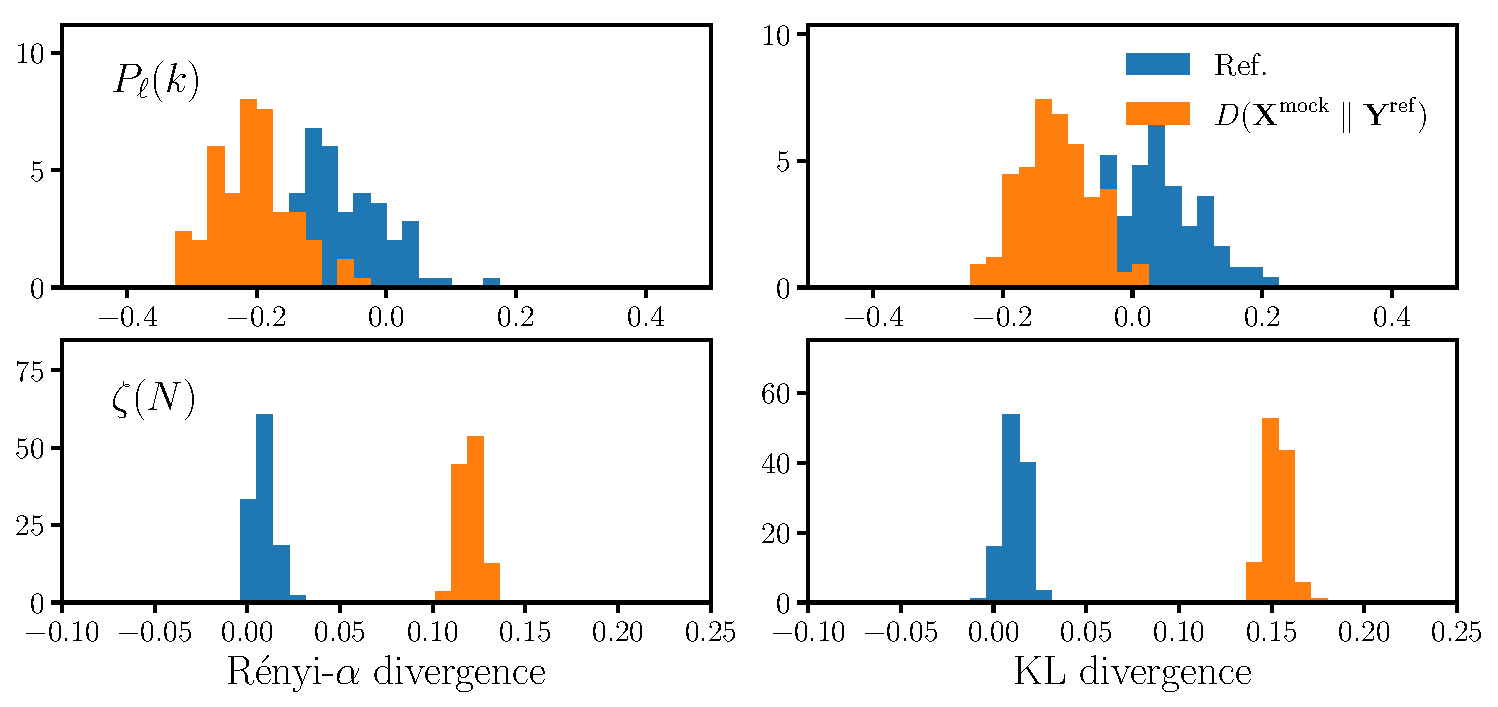
\includegraphics[width=0.9\textwidth]{figs/kNNdiverg_Gauss.pdf}
    \caption{R\'enyi-$\alpha$ and KL divergence estimates 
    ($\hat{D}_{R\alpha}$ and $\hat{D}_{KL}$; orange) between 
    the likelihood distribution and the Gaussian pseudo-likelihood 
    for the \Beut~$P_\ell$ (top) and \Sinh~$\zeta$ (bottom) analyses. 
    We include in blue, as reference, the divergence estimates 
    of the pseudo-likelihood onto itself.  
    $\hat{D}_{R\alpha}$ and $\hat{D}_{KL}$ are computed using the 
    non-parametric $k$-NN estimator (Section~\ref{sec:div}) on 
    the mock data $\Xmock$ and a referece sample $\Yref$ drawn
    from the pseudo-likelihood. We compute $\hat{D}_{R\alpha}$ and
    $\hat{D}_{KL}$ \todo{100} times and plot their distribution 
    in order to illustrate the uncertainty in the $\hat{D}$ 
    estimator. The significant discrepancy between 
    the two divergence distributions in each of the panels, identifies 
    the \emph{significant non-Gaussianity of the $P_\ell(k)$ and $\zeta(N)$ 
    likelihoods}. 
    }
\label{fig:div_gauss}
\end{center}
\end{figure}
%%%%%%%%%%%%%%%%%%%%%%%%%%%%%%%%%%%%%

\section{Estimating the Non-Gaussian Likelihood} \label{sec:likeest}
In the previous section, we estimate the divergence between the 
$P_\ell$ and $\zeta$ likelihoods sampled by mocks and their respective 
Gaussian pseudo-likelihoods. These divergences identify and quantify 
the significant non-Gaussianity in the likelihoods of LSS studies.   
Our ultimate goal, however, is to quantify the impact of likelihood 
non-Gaussianity on the final cosmological parameter constrains and
to develop more accurate methods for parameter inference in LSS. 
From the divergence estimates alone, it's not obvious how they propagate 
onto the final parameter constraints. Therefore in this section, 
we present two methods for more accurately estimating the non-Gaussian 
likelihoods of $P_\ell$ and $\zeta$ from the corresponding mocks.
These methods provide a more accurate estmiate of the likelihood than 
the Gaussian pseudo-likelihood. Moreover, we will use them later to 
quantify the impact of likelihood non-Gaussianity on the 
\Beut~and \Sinh~parameter constraints. 

\subsection{Gaussian Mixture Likelihood Estimation} \label{sec:gmm}
When mock catalogs are used for parameter inference in LSS analyses, 
they essentially serve as data points sampling the likelihood distribution. 
For the pseudo-likelihood, this distribution is assumed to have a 
Gaussian functional form. Hence, why we estimate the covariance matrix 
from mocks. However, the Gaussian functional form, or any functional form for 
that matter, is \emph{not} necessary to estimate the likelihood distribution. 
Instead, the multidimensional likelihood distribution 
can be directly estimated from the set of mock catalogs using --- for 
instance using Gaussian mixture density 
estimation~\citep{Press:1992:NRC:148286,9780471006268}. 
Besides its extensive use in machine learning and statistics, 
in astronomy, Gaussian mixture density estimation has been used for 
inferring the velocity distribution of stars from the Hipparcos 
satellite~\citep{bovy2011}, classifying galaxies in the Galaxy And Mass Assembly 
Survey~\citep{taylor2015}, and classifying pulsars~(\citealt{lee2012}; see
also~\citealt{hogg2010,kuhn2017}). 

Gaussian mixture density estimation is a ``semi-parametric'' method 
that uses a weighted sum of $k$ Gaussian component densities, a Gaussian 
mixture model (hereafter GMM)
\beq
p(x; \bm{\theta}) = \sum\limits_{i=1}^{k} \pi_i\, \mathcal{N}(x; \bm{\theta}_i),
\eeq
to estimate the density. 
The component weights ($\pi_i$; also known as mixing weights) and the 
component parameters $\bm{\theta}_i$ are free parameters of the mixture 
model. Given some data set ${\bf X}_N = \{{\bf x}_1,..., {\bf x}_N \}$, 
these free GMM parameters are, most popularly, estimated 
through an expectation-maximization algorithm~\citep[EM;][]{dempster1977, neal1998}.
The EM algorithm begins by randomly assigning $\bm{\theta}^0_i$ to the 
$k$ Gaussian components. The algorithm then iterates between two steps. 
In the first step, the algorithm computes for each data point, ${\bf x}_n$, 
a probability of being generated by each component of the model. These 
probabilities can be thought of as weighted assignments of the points 
to the components. Next, given the ${\bf x}_n$ assignment to the 
components, $\bm{\theta}^t_i$ of each component are updated to $\bm{\theta}^{t+1}_i$
to maximize the likelihood of the assigned points. At this point, $\pi_i$ 
can also be updated by summing up the assignment weights and 
normalizing it by the total number of data points, $N$. This entire
process is repeated until convergence --- \emph{i.e.} when the log-likelihood of 
given the mixture model $\log\,p({\bf X}_N; \bm{\theta}^t)$ %= \sum\limits_{n=1}^{N} \log\,p({\bf x}_n; \bm{\theta}^t)
converges. The EM algorithm is guaranteed to converges to a local maximum 
of the likelihood~\citep{wu1983}. 

In practice, instead of arbitrarily assigning the initial condition, 
$\bm{\theta}^0_i$ is derived from a $\mathtt{k}$-$\mathtt{means}$ 
clustering algorithm~\citep{lloyd1982}. Without going into details, the 
$\mathtt{k}$-$\mathtt{means}$ algorithm clusters the data ${\bf X}_N$ into $k$ 
clusters, each described by the mean (or centroid) $\mu_i$ of the
samples in the cluster. The algorithm then iteratively chooses centroids that 
minimize the average squared distance between points in the same cluster.
For our GMMs, we set the initialize the EM algorithm using 
the $\mathtt{k}$-$\mathtt{means}{\tiny ++}$ algorithm of ~\cite{arthur2007}. 
In Figure~\ref{fig:gmm_ped}, we illustrate Gaussian mixture 
density estimation in action. We use GMMs with $k = 1$ (top), $
3$ (middle), and $10$ (bottom) components to estimate the
distribution of one dimensional data (blue) drawn from three 
separate Gaussian distributions. The GMM outputs of the EM algorithm 
are plotted in red with dotted black lines representing each of their 
components.  

%%%%%%%%%%%%%%%%%%%%%%%%%%%%%%%%%%%%%
% Figure 2 
%%%%%%%%%%%%%%%%%%%%%%%%%%%%%%%%%%%%%
\begin{figure}
\begin{center}
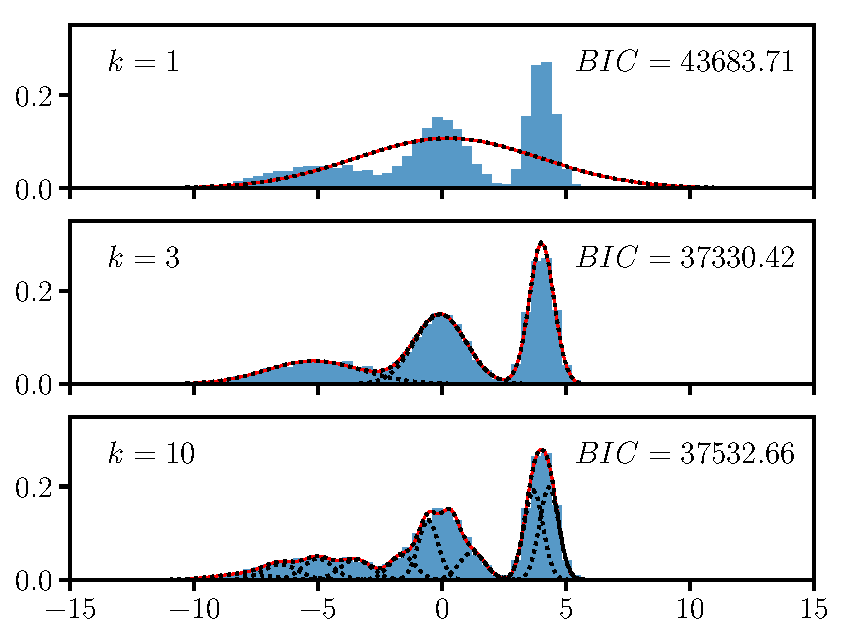
\includegraphics[width=0.65\textwidth]{figs/GMM_pedagog.pdf}
\caption{A pedagogical illustration of Gaussian mixture density estimation.
    We use GMMs with $k = 1$ (top), $3$ (middle), $10$ (bottom) 
    components to estimate the distribution of data (blue) drawn from three 
    Gaussian distributions. The GMM outputs of the EM algorithm 
    are plotted in red with \todo{dotted lines} representing each of their 
    components (Section~\ref{sec:gmm}). We also include the BIC of 
    the GMMs, which we use to select the number of components $k$. 
    Of the three panels, $k=3$ has the lowest BIC and therefore 
    best represents the data according to our selection scheme.} 
\label{fig:gmm_ped}
\end{center}
\end{figure}
%%%%%%%%%%%%%%%%%%%%%%%%%%%%%%%%%%%%%

So far in our description of GMMs, we have kept
the number of components $k$ fixed. However, $k$ is a free 
parameter and selecting it is a crucial step in Gaussian mixture
density estimation. With too many components the model may overfit 
the data; with too few components, 
the model may not be flexible enough to approximate the true 
underlying distribution. In order to address this model selection problem
of selecting $k$, we make use of the Bayesian Information 
Criterion~\citep[BIC;][]{schwarz1978}. BIC has been widely used for 
determining the number of components in mixture 
modeling~\citep[\emph{e.g.}][]{leroux1992,roeder1997,fraley1998,steele2010performance}
and for model selection in general in 
astronomy~\citep[\emph{e.g.}][]{liddle2007,broderick2011,wilkinson2015,vakili2016}.
According to BIC, models with higher likelihood are preferred; however, 
to address the concern of overfitting, BIC introduces a \emph{penalty} term 
for the number of parameters in the model: 
\beq \label{eq:bic}
\mathrm{BIC} = -2\,\mathrm{ln}\,\mathcal{L} + N_\mathrm{par}\,\mathrm{ln}\,N_\mathrm{data}.
\eeq
We select $k$ based on the number of components in the model with the 
lowest BIC. Of the three panels in Figure~\ref{fig:gmm_ped}, the GMM 
model with $k=3$ components has the lowest BIC and therefore would be 
selected. At least in this example, the choice of $k=3$ is 
obviously justified. The $k = 1$ GMM is definitely not flexible enough 
to characterize the underlying distribution and the $k=10$ GMM clearly
overfits the distribution. 

With Gaussian mixture density estimation we can directly estimate 
the likelihood distribution using the mock catalogs. We first fit 
GMMs with $k\mathrm{s} < 30$ components to the whitened 
mock data $\Xmock$ using the EM algorithm for each model. For each of the 
converged GMMs, we calculate the BIC. Afterwards we select 
the model with the lowest BIC as the best density estimate of the likelihood 
distribution: $\hat{p}_\mathrm{\tiny GMM}(x)$. The selected density estimate can 
then be used to calculate the
likelihood and quantify the impact of likelihood non-Gaussianity on the 
parameter constraints of~\Beut~and~\Sinh. But before we do that, we have to 
confirm whether $\hat{p}_\mathrm{\tiny GMM}$ is in fact a better estimate 
of the likelihood over the Gaussian pseudo-likelihood. To do this, we return 
to the divergence estimates of Section~\ref{sec:div}. 

To estimate the divergence between our Gaussian mixture density estimate,
$\hat{p}_\mathrm{\tiny GMM}$, and the likelihood distribution, we take 
the same approach as our $\hat{D}$ calculation in Section~\ref{sec:div}. 
Instead of $\Yref$ drawn from the pseudo-likelihood, we draw 
samples from $\hat{p}_\mathrm{\tiny GMM}(x)$ with the same 
dimensions. Then we calculate $k$-NN~\Ralpha~and KL 
divergence estimates between this sample and $\Xmock$. As we did in Figure~\ref{fig:div_gauss}, 
we repeat this process \todo{100} times, resampling $\hat{p}_\mathrm{\tiny GMM}$
each time, in order get a distribution of divergence estimates that 
reflects the scatter in the estimator. In Figure~\ref{fig:div_gmm}, 
we present the resulting distribution of divergences between 
$\hat{p}_\mathrm{\tiny GMM}$ and the likelihood distribution in \todo{green} 
for the $P_\ell(k)$ (top) and $\zeta(N)$ (bottom) analyses. For comparison, 
we include the distributions from Figure~\ref{fig:div_gauss}. 

For the $\zeta(N)$ analysis of \Sinh, our Gaussian mixture density 
estimate significantly improves the divergence discrepancy compared to the 
pseudo-likelihood. In other words, \emph{our Gaussian mixture density estimate  
is a significant better estimate of the $\zeta$ likelihood distribution
than the pseudo-likelihood}. On the other hand, our Gaussian mixture 
density estimate for the $P_\ell(k)$ analysis of \Beut~does not 
significantly improve the divergence discrepancy. This difference in 
the performance of Gaussian mixture density estimation is not surprising. 
One would expect a direct density estimation to be more effective 
for the \Sinh~case, where we estimate an $8$-dimensional 
distribution with $N_\mathrm{mock} = 20,000$ samples, compared to the \Beut~ 
case where we estimate a $37$-dimensional distribution with 
only $N_\mathrm{mock} = 2048$ samples. 
Given the unconvincing accuracy of the Gaussian mixture density estimate
of the $P_\ell$ likelihood, in the next section we present an alterative 
method for estimating the non-Gaussian likelihood.

%%%%%%%%%%%%%%%%%%%%%%%%%%%%%%%%%%%%%
% Figure 3 
%%%%%%%%%%%%%%%%%%%%%%%%%%%%%%%%%%%%%
\begin{figure}
\begin{center}
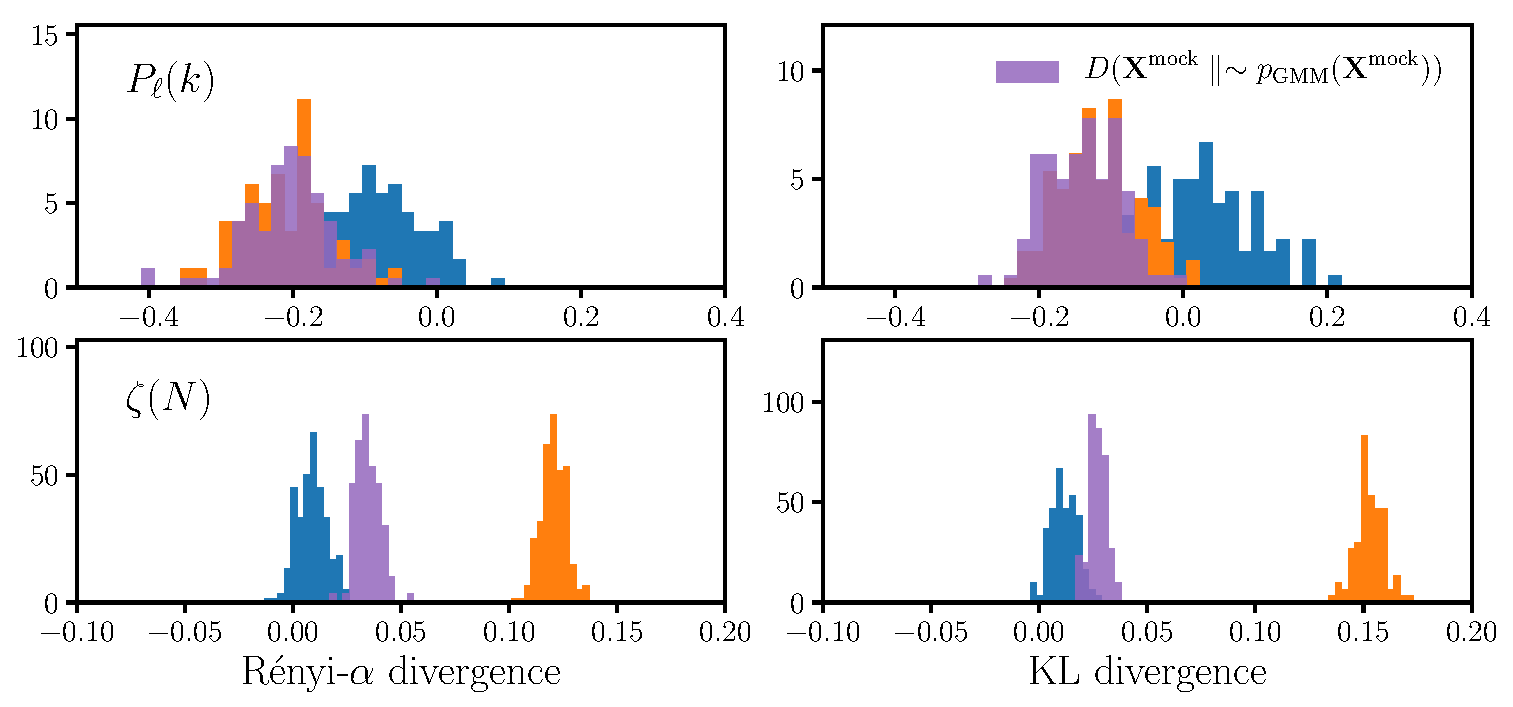
\includegraphics[width=0.9\textwidth]{figs/kNNdiverg_gmm.pdf}
\caption{R\'enyi-$\alpha$ and KL divergence estimates 
    ($\hat{D}_{R\alpha}$ and $\hat{D}_{KL}$; \todo{green}) between 
    the likelihood distribution and the Section~\ref{sec:gmm} GMM 
    likelihood estimate for the \Beut~$P_\ell$ (top) and \Sinh~$\zeta$ 
    (bottom) analyses. We include the divergence estimates from 
    Figure~\ref{fig:div_gauss} for comparison. The Gaussian mixture
    likelihood does not significantly improve the discrepancy in 
    divergence for the $P_\ell$ analysis. This is due to the high-dimensionality 
    (37 dimensions) of the $P_\ell$ likelihood. However, for the $\zeta$ 
    analysis, \emph{our Gaussian mixture likelihood estimate is 
    a significantly better estimate of the likelihood
    than the pseudo-likelihood.}
    }
\label{fig:div_gmm}
\end{center}
\end{figure}
%%%%%%%%%%%%%%%%%%%%%%%%%%%%%%%%%%%%%

\subsection{Independent Component Analysis} \label{sec:ica}
Gaussian mixture density estimation fails to accurately estimate 
the $37$-dimensional $P_\ell$ likelihood distribution of \Beut. 
Rather than estimating the likelihood distribution directly, 
if we can transform the observable ${\bf x}$ (\emph{e.g.} $P_\ell$) 
into statistically independent components ${\bf x}^\mathrm{IC}$ 
the problem becomes considerably simpler. Since ${\bf x}^\mathrm{IC}$ 
is statistically independent the likelihood distribution becomes 
\beq \label{eq:ica_like}
p(x) = \prod\limits_{n=1}^{N_\mathrm{bin}} p_{x^\mathrm{IC}_n} (x) 
\eeq
where $N_\mathrm{bin}$ is the number of bins in the observable. 
For the \Beut~case, this reduces the problem of estimating a 37 
dimensional distribution with $2048$ samples to a problem of 
estimating 37 one dimensional distributions with $2048$ samples 
each. The challenge, however, is in finding the transformation. 

Efforts in the past have attempted to tackle this sort of 
high-dimensional problem~\citep[\emph{e.g.}][]{scoccimarro2000,eisenstein2001,gaztanaga2005,norberg2009,sinha2017a}.
They typically use singular value decomposition or principal 
component analysis~\citep[PCA;][]{Press:1992:NRC:148286}. For a Gaussian
likelihood, the PCA components of it are statistically independent. 
However, when the likelihood is \emph{not} Gaussian, the PCA components 
are uncorrelated but~\emph{not necessarily statistically independent}~\citep{hartlap2009}. 
Since the $P_\ell$ and $\zeta$ likelihoods are non-Gaussian, we cannot 
use PCA. Instead, we follow \cite{hartlap2009} and use Independent 
Component Analysis~\citep[ICA][]{herault1984,comon1994,hyvarinen2000,
hyvarinen2001independent}. 

In order to find the transformation of ${\bf x}$ to ${\bf x}^\mathrm{IC}$ 
we first assume that ${\bf x}$ is generated by some linear transformation
${\bf x} = {\bf M}\,{\bf x}^\mathrm{IC}$. The goal of ICA is to invert 
this problem, ${\bf y} = {\bf W}\,{\bf x}$, and find ${\bf W}$ and ${\bf y}$ 
that best estimate ${\bf y} \approx {\bf x}^\mathrm{IC}$. The basic 
premise of ICA is simple, \emph{maximizing non-Gaussianity maximizes the 
statistical independence}. Consider a single component of ${\bf y}$: 
\beq
{\bf y}_n = {\bf w}_n^{\tiny t}\,{\bf x} = {\bf w}_n^{\tiny t}\,{\bf M}\,{\bf x}^\mathrm{IC} 
\eeq
where ${\bf w}_n^{\tiny t}$ is the $n^\mathrm{th}$ row of ${\bf W}$. 
Since ${\bf y}_n$ is a linear combination of the independent 
components ${\bf x}^\mathrm{IC}$, due to the Central Limit Theorem 
${\bf y}_n$ is necessarily more Gaussian than any of the 
components \emph{unless} ${\bf y}_n$ is equal to one of the 
${\bf x}^\mathrm{IC}$ components. In other words, we can achieve 
${\bf y} \approx {\bf x}^\mathrm{IC}$ by finding ${\bf W}$ that 
maximizes the non-Gaussianity of ${\bf y}$. For a more rigorous 
justification of ICA we refer readers to~\cite{hyvarinen2001independent}. 
In practice, non-Gaussianity is commonly measured using differential
entropy --- ``negentropy''. For ${\bf y}_n$ with density function 
$p_{y_n}$ the entropy is defined as
\beq
H_{y_n} =  - \int p_{y_n} (y)\, \log p_{y_n}(y)\, \mathrm{d}y. 
\eeq
Since the Gaussian distribution has the largest entropy among all 
distributions with a given variance, the negentropy can be defined 
as, 
\beq
J_{y_n} = H_{y_n^\mathrm{Gauss}} - H_{y_n}. 
\eeq
Finding the statistically independent components is now a matter
of finding the ${\bf W}$ that maximizes $\sum\limits_{n} J_{\bf y_n}$
--- the negentropy of ${\bf y}$. In this paper, we make use of the 
$\mathtt{FastICA}$ fixed-point iteration algorithm~\citep{hyvarinen1999}. 
The algorithm starts with randomly selected ${\bf w}_ns$, then it uses 
approximations of negentropy from~\cite{hyvarinen1998} and Newton's method 
to iteratively solve for ${\bf W}$ that maximizes negentropy. For details 
on the $\mathtt{FastICA}$ algorithm, we refer readers to~\cite{hyvarinen1999}.

Performing ICA on the whitened observable data $\Xmock$, we derive the 
matrix ${\bf W}$ that transforms $\Xmock$ into $N_\mathrm{bin}$
approximately independent components: 
\beq
{\bf X}^\mathrm{ICA} = {\bf W}\,\Xmock = \{{\bf X}^\mathrm{ICA}_1, ..., {\bf X}^\mathrm{ICA}_{N_\mathrm{bin}}\}.
\eeq
From these statistically independent components and Eq.~\ref{eq:ica_like}, 
we can estimate the likelihood distribution. $p_{x^\mathrm{IC}_n} (x)$, 
from Eq.~\ref{eq:ica_like}, is the 1-dimensional distribution 
function of the $n^\mathrm{th}$ ICA component. This distribution 
is sampled by ${\bf X}^\mathrm{ICA}_n$, the transformed mock data. 
That means ${\bf X}^\mathrm{ICA}_n$ can be used to estimate 
$p_{x^\mathrm{ICA}_n}$ using a method like kernel 
density estimation~\citep[KDE; \emph{e.g.}][]{9780387848587,feigelson2012}. 
With KDE, the density estimate, $\hat{p}_{x^\mathrm{ICA}_n}$, is constructed by 
smoothing the empirical distribution of the ICA component $x^\mathrm{ICA}_n$ 
using a smooth kernel: 
\beq
\hat{p}_{x^\mathrm{ICA}_n}(x) = \frac{1}{N_\mathrm{mock}b} \sum\limits_{j=1}^{N_\mathrm{mock}} K \left( \frac{x - \mathrm{X}^{(j),\mathrm{ICA}}_n}{b} \right). 
\eeq
$b$ is the bandwidth and $K$ is the kernel function. Following the 
choices of \cite{hartlap2009}, we use a Gaussian distribution for $K$ and the 
``rule of thumb'' bandwidth~\cite[also known as Scott's rule;][]{scott1992,davison2008} 
for $b$. Combining $\hat{p}_{x^\mathrm{ICA}_n}s$ estimates for 
all $n = 1, ..., N_\mathrm{bin}$ into Eq.~\ref{eq:ica_like}, we 
can estimate the likelihood distribution $p(x) \approx \prod\limits_n \hat{p}_{x^\mathrm{ICA}_n}(x)$

We again test whether the likelihood estimate from ICA is actually 
a better estimate of the likelihood distribution than the Gaussian 
pseudo-likelihood. Following the same procedure as we 
did for the Gaussian mixture likelihood in Section~\ref{sec:gmm}, we 
calculate the divergence between our ICA likelihood, $\prod \hat{p}_{x^\mathrm{ICA}_n}(x)$, 
and the likelihood distribution, $p(x)$. We draw a sample from 
$\prod \hat{p}_{x^\mathrm{ICA}_n}$ with the same dimensions as 
$\Yref$ (Section~\ref{sec:div}), apply the mixing matrix 
(undoing the ICA transformation), and then calculate the 
$k$-NN~\Ralpha~and KL divergence estimates between the sample and $\Xmock$. 
We repeat these steps \todo{100} times to get the distribution of estimates 
that reflects the scatter in the estimator. In Figure~\ref{fig:div_ica}, 
we present the resulting distribution of 
$\hat{D}\left(\Xmock \parallel \sim \prod \hat{p}_{x^\mathrm{ICA}_n} \right)$
in \todo{green} for the $P_\ell(k)$ (top) and $\zeta(N)$ (bottom) analyses. 
For comparison, we include the distributions from Figure~\ref{fig:div_gauss}. 

%%%%%%%%%%%%%%%%%%%%%%%%%%%%%%%%%%%%%
% Figure 4 
%%%%%%%%%%%%%%%%%%%%%%%%%%%%%%%%%%%%%
\begin{figure}
\begin{center}
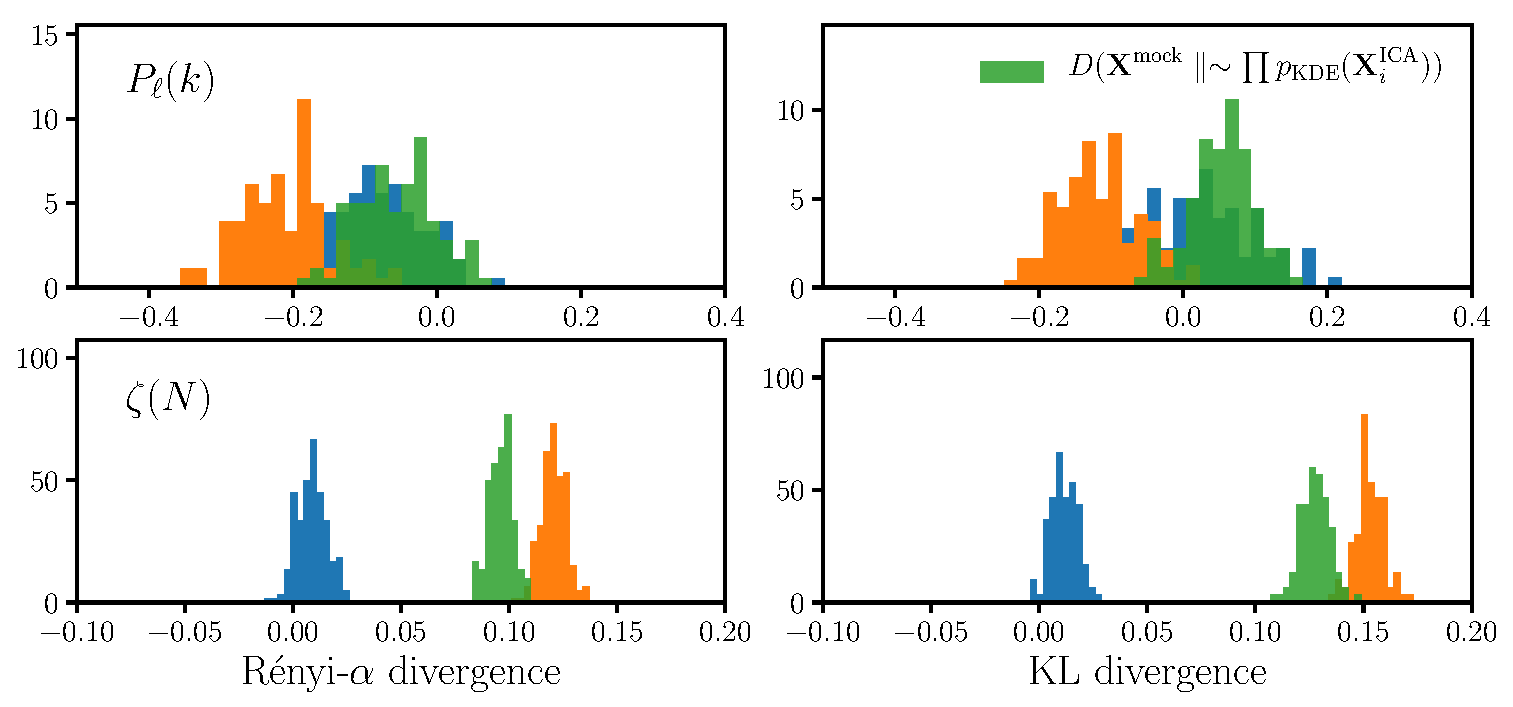
\includegraphics[width=0.9\textwidth]{figs/kNNdiverg_ica.pdf}
\caption{R\'enyi-$\alpha$ and KL divergence estimates 
    ($\hat{D}_{R\alpha}$ and $\hat{D}_{KL}$; \todo{green}) between 
    the likelihood distribution and the Section~\ref{sec:ica} ICA 
    likelihood estimate for the \Beut~$P_\ell$ (top) and \Sinh~$\zeta$ 
    (bottom) analyses. We include the divergence estimates from 
    Figure~\ref{fig:div_gauss} for comparison. The ICA likelihood 
    significantly improves the divergence discrepancy for both the
    $P_\ell$ and $\zeta$ analyses. For $\zeta$, the improvement of 
    the ICA likelihood over the pseudo-likelihood is more modest than 
    our GMM estimate from Section~\ref{sec:gmm}. However, for 
    $P_\ell$, where the GMM method struggled, our ICA likelihood 
    provides a significant improvement.
    }
\label{fig:div_ica}
\end{center}
\end{figure}
%%%%%%%%%%%%%%%%%%%%%%%%%%%%%%%%%%%%%

For \emph{both} \Beut~and~\Sinh, our ICA likelihood significantly 
improves the divergence discrepancy compared to the pseudo-likelihood. For 
\Sinh, however, the ICA likelihood proves to be less accurate than 
the Gaussian mixture likelihood in Section~\ref{sec:gmm}. More importantly, 
for \Beut, where the Gaussian mixture likelihood did not improve 
upon the pseudo-likelihood, the ICA method provides a significantly 
more accurate likelihood estimate. This demonstrates that the ICA 
method is an alterative to the more direct Gaussian mixture method. 
Furthermore, the effectiveness of the ICA method in estimating
higher dimensional likelihoods with fewer samples (mocks) is  
particularly appealing for LSS, since analyses continue to 
increase the size of their observable data vector. However, as 
the divergence estimation framework we present makes it easy to test the accuracy of different methods, a hard 
choice is not necessary and multiple methods can easily be tested to construct 
the best estimate of the likelihood distribution for each specific analysis. 
Based on the performances of the GMM and ICA methods, in the following
sections we use the ICA method for the~\Beut~analysis and the GMM 
method for the~\Sinh~analysis. 

\section{Impact on Parameter Inference}
To derive the posterior distribution of their model parameters,
both~\Beut~and~\Sinh~use the standard Monte Carlo Markov Chain (MCMC) 
approach with the Gaussian pseudo-likelihood. The \Beut~analysis 
includes $11$ parameters,
\beq \nonumber
\Big \{f \sigma_8,~\alpha_\parallel,~\alpha_\perp,~b_1^\mathrm{NGC} \sigma_8,~b_1^\mathrm{SGC} \sigma_8, 
~b_2^\mathrm{NGC} \sigma_8,~b_2^\mathrm{SGC} \sigma_8,~\sigma_v^\mathrm{NGC},~\sigma_v^\mathrm{SGC}, 
~N^\mathrm{NGC},~\mathrm{and}~N^\mathrm{SGC} \Big \}, 
\eeq
while the \Sinh~analysis includes $5$ parameters,
\beq \nonumber
\Big\{ \log\,M_\mathrm{min},~\sigma_{\log\,M},~\log\,M_0,~\log\,M_1,~\mathrm{and}~\alpha \Big\}. 
\eeq
Using the improved likelihood estimates of Sections~\ref{sec:gmm} 
and~\ref{sec:ica}, we can now better estimate the true posterior distributions
of these parameters and quantify the impact of likelihood non-Gaussianity 
on parameter constraints. The most straightforward 
approach to do this would be to use the likelihood estimates to compute 
MCMC samples from scratch. While this is relatively doable for the~\Beut~analysis, 
for~\Sinh~this is \emph{significantly} more involved. Rather than a perturbation 
theory based model from~\Beut, the \Sinh~model is a forward model, same as 
their mocks (Section~\ref{sec:gmf}). Rerunning the MCMC samples would involve
evaluating their computationally costly forward model $> 10^5$ times. 

Without having to re-run the MCMC chains, we instead use importance sampling 
to derive the new posteriors from the original chains~\citep[see][for details on importance sampling]{wasserman2004}. 
The \emph{target} distribution we want is the new posterior. To sample this 
distribution, we sample the original posterior as the \emph{proposal} 
distribution with importance weights, which in our case is the ratio 
of our likelihood estimates over the pseudo-likelihood. If we let 
$P({\bf x} | \bm{\theta})$ be the original pseudo-likelihood and 
$P'({\bf x} | \bm{\theta})$ be our ``new'' likelihood, then the new 
marginal likelihood can be calculated through importance sampling:   
\beq
P'({\bf x} | \theta_1) = \int P'({\bf x} | \bm{\theta})\,\mathrm{d}\theta_2...\mathrm{d}\theta_m = \int \frac{P'({\bf x} | \bm{\theta})}{P({\bf x} | \bm{\theta})}\, P({\bf x} | \bm{\theta})\,\mathrm{d}\theta_2...\mathrm{d}\theta_m \\
\eeq
Through Monte Carlo integration, this becomes 
\beq
P'({\bf x} | \theta_1) \approx \sum\limits_{\bm{\theta}^{(i)} \in S} \frac{P'({\bf x} | \bm{\theta}^{(i)})}{P({\bf x} | \bm{\theta}^{(i)})}. \label{eq:impsamp}
\eeq
where $S$ is the sample drawn from $P({\bf x} | \bm{\theta})$. In our 
case $S$ is just the original MCMC chain. The only calculation required 
is the importance weights in Eq.~\ref{eq:impsamp}, 
${P'({\bf x} | \bm{\theta}^{(i)})}/{P({\bf x} | \bm{\theta}^{(i)})}$ for 
each sample $\bm{\theta}^{(i)}$ of the original MCMC chain. 
For \Beut, $P({\bf x} | \bm{\theta}^{(i)})$ is the ICA likelihood;  
for \Sinh, $P({\bf x} | \bm{\theta}^{(i)})$ is the GMM likelihood.

We present in Figure~\ref{fig:pk_like} the resulting posterior 
distributions using the non-Gaussian ICA likelihood for the 
$\big \{f \sigma_8$, $\alpha_\parallel$, $\alpha_\perp$, 
$b_1^\mathrm{NGC} \sigma_8$, $b_1^\mathrm{SGC} \sigma_8$, 
$b_2^\mathrm{NGC} \sigma_8$, $b_2^\mathrm{SGC} \sigma_8,\big \}$
parameters in the \Beut~$P_\ell$ analysis (orange). We include 
the original~\Beut~posteriors for comparison in blue. On the 
bottom of each panel, we also include box plots marking the 
confidence intervals of the updated and original posteriors. 
The boxes and ``whiskers'' repesent the $68\%$ and $95\%$ 
confidence intervals, respectively. The median and $68\%$ 
confidence intervals of the posteriors are listed in Table~\ref{tab:posterior}.
$f \sigma_8$ and $b_2^\mathrm{SGC} \sigma_8$ are the main parameters with 
noticeable change in their posteriors. The posterior of $b_2^\mathrm{SGC} \sigma_8$
broadens from $0.476^{+1.262}_{-1.175}$ to $0.422^{+1.517}_{-1.377}$ once likelihood 
non-Gaussianity is incorporated. Meanwhile, the $f \sigma_8$ posterior
shifts from $0.478^{+0.053}_{-0.049}$ to $0.456^{+0.059}_{-0.049}$, which 
corresponds to a  shift of $0.44 \sigma$. The other parameter constraints, 
however, remain largely unaffected by likelihood non-Gaussianity. 

Focusing on the main cosmological parameters $f \sigma_8$, 
$\alpha_\parallel$, and $\alpha_\perp$, we present their 
joint posterior distributions in Figure~\ref{fig:rsd_contour}.  
The contours mark the $68\%$ and $95\%$ confidence intervals
of the posteriors. The shift in the $f \sigma_8$ distribution 
is reflected in the
$(f\sigma_8, \alpha_\parallel)$ and $(\alpha_\perp, f\sigma_8)$ 
contours (left and middle panels respectively). The 
$(\alpha_\parallel, \alpha_\perp)$ distribution (right), however, show nearly 
no change from the non-Gaussian likelihood. %These joint posteriors corroborate our conclusion from Figure~\ref{fig:pk_like}.
Despite its impact on $f \sigma_8$ and $b_2^\mathrm{SGC} \sigma_8$, 
overall, likelihood non-Gaussianity does \emph{not}
significantly impact the parameter constraints of the $P_\ell$ 
analysis. $b_2^\mathrm{SGC} \sigma_8$ is a poorly constrained nuisance 
parameter. Although using the pseudo-likelihood biases $f \sigma_8$, 
the impact relative to its uncertainty is small --- less than $0.5 \sigma$. 
The fact that the $P_\ell$ analysis is largely unaffected by likelihood 
non-Gaussianity is consistent with the divergences in 
Figure~\ref{fig:div_gauss}, which found relatively small discrepancies 
between the likelihood and pseudo-likelihood. 

%Furthermore, the Gaussian pseudo-likelihood assumption for $P_\ell$ 
%is motivated by the Central Limit Theorem: if enough modes contribute  
%to the powerspectrum, then the likelihood approaches a Gaussian. In 
%the restrictive $k$ range of the \Beut~analysis ($0.01 < k < 0.15$), 
%one would expect this to be the case. 
%\todo{When we repeat the comparison for the $P_\ell$ analysis without 
%the hexadecapole, we see even less impact on the parameter constraints. 
%This suggests that most of the non-Gaussianity in the likelihood comes 
%from the hexadecapole which has the lowest signal to noise.} 

%%%%%%%%%%%%%%%%%%%%%%%%%%%%%%%%%%%%%
% Figure 5 
%%%%%%%%%%%%%%%%%%%%%%%%%%%%%%%%%%%%%
\begin{figure}
\begin{center}
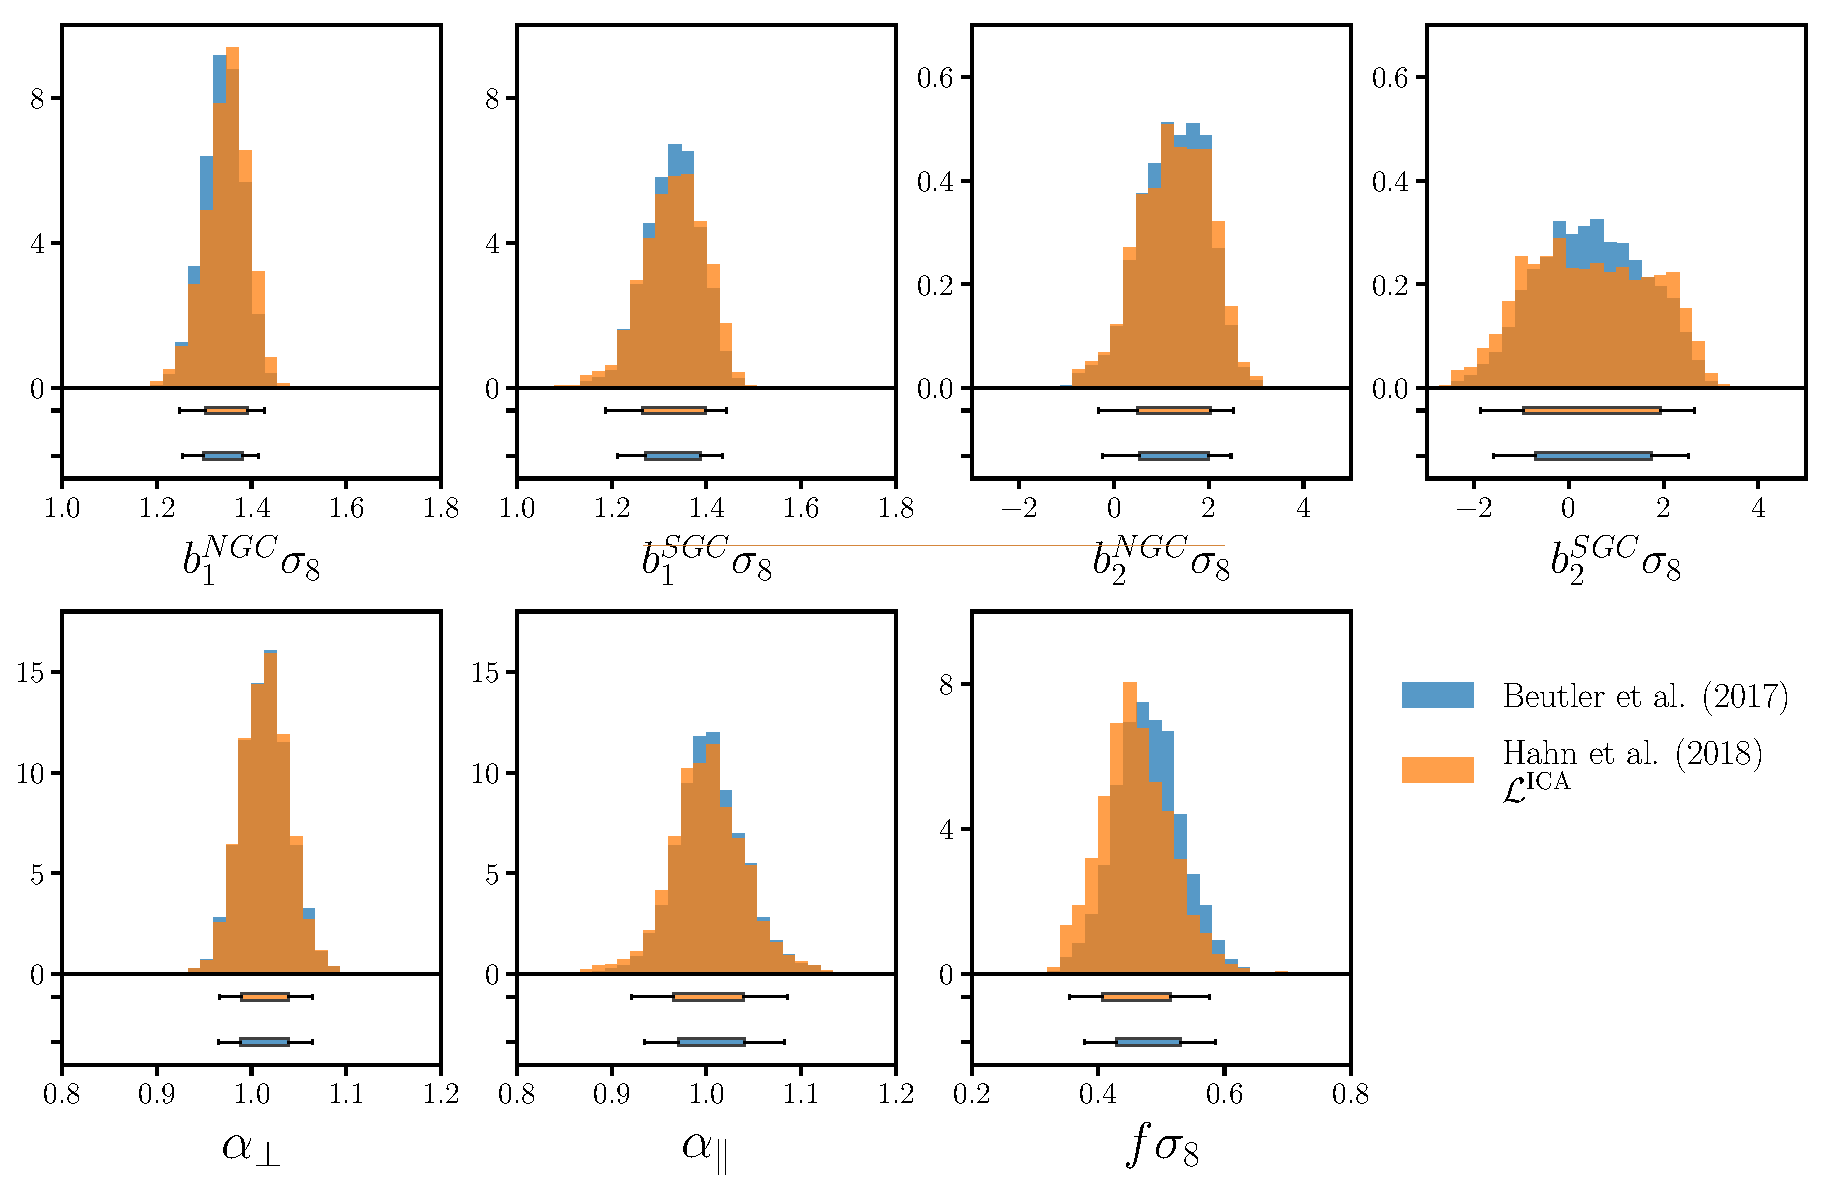
\includegraphics[width=\textwidth]{figs/Like_Pk_comparison.pdf}
\caption{The posterior distribution for 
    $\big \{f \sigma_8$, $\alpha_\parallel$, $\alpha_\perp$, 
    $b_1^\mathrm{NGC} \sigma_8$, $b_1^\mathrm{SGC} \sigma_8$, 
    $b_2^\mathrm{NGC} \sigma_8$, $b_2^\mathrm{SGC} \sigma_8,\big \}$ 
    in the~\Beut~$P_\ell$ analysis using the non-Gaussian ICA 
    likelihood (orange). We include in blue the original~\Beut~posteriors 
    for comparison. On the bottom of each panel we include box 
    plots that mark the $68\%$ and $95\%$ confidence intervals of
    the posterior. The discrepancy between the posteriors is most 
    evident for the parameters $f\sigma_8$ and and $b^\mathrm{SGC}_2 \sigma_8$.  
    Hence, using the pseudo-likelihood in the $P_\ell$ analysis 
    biases the posteriors of these parameters. 
    Overall, however, likelihood non-Gaussianity does \emph{not} 
    have a siginificant impact on the parameter constraints of 
    the $P_\ell$ analysis.} 
\label{fig:pk_like}
\end{center}
\end{figure}
%%%%%%%%%%%%%%%%%%%%%%%%%%%%%%%%%%%%%


%%%%%%%%%%%%%%%%%%%%%%%%%%%%%%%%%%%%%
% Figure 6 
%%%%%%%%%%%%%%%%%%%%%%%%%%%%%%%%%%%%%
\begin{figure}
\begin{center}
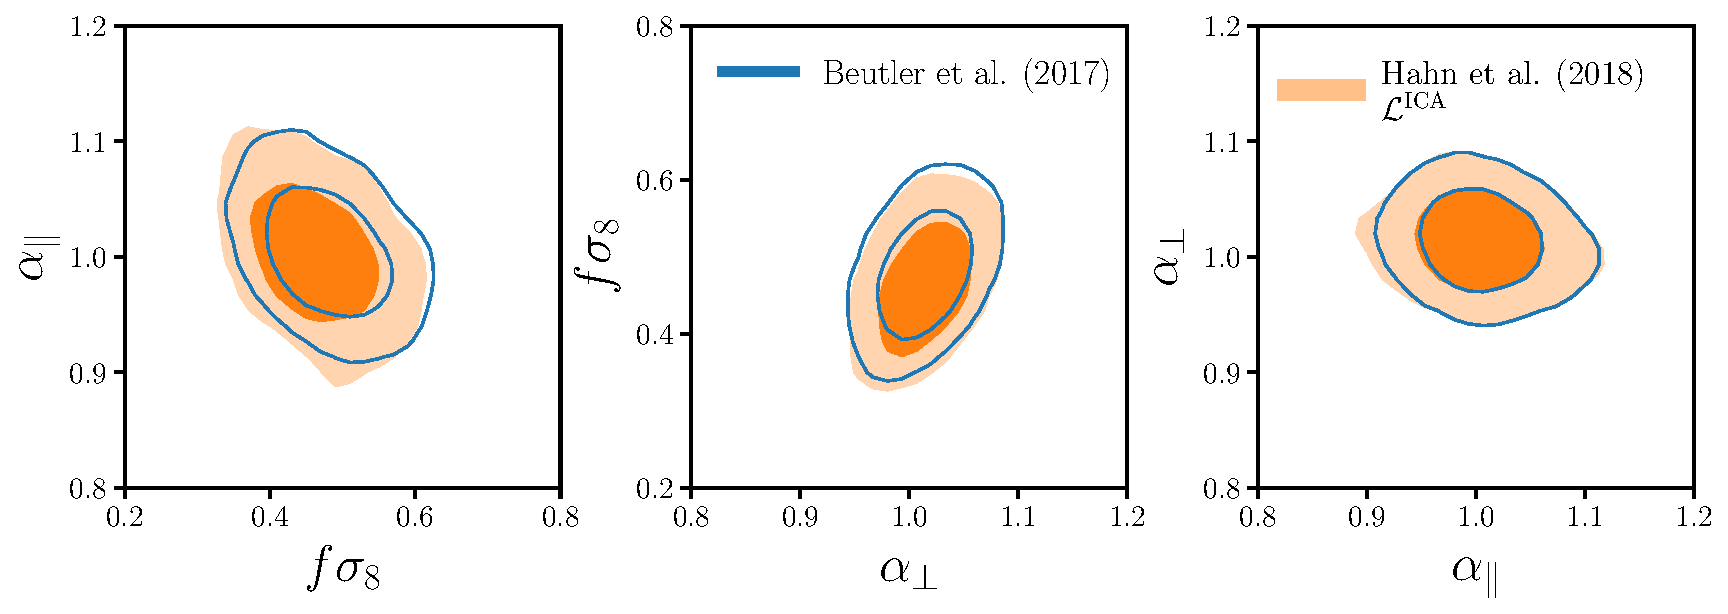
\includegraphics[width=\textwidth]{figs/RSD_contours.pdf}
\caption{Joint posterior distributions of $f \sigma_8$, 
    $\alpha_\parallel$, and $\alpha_\perp$ in the~\Beut~$P_\ell$ 
    analysis, compute using the non-Gaussian ICA likelihood (orange). 
    We include, in blue, the original~\Beut~posteriors for comparison. 
    The contours in the left and middle panels reflect the shift
    in $f \sigma_8$ caused by likelihood non-Gaussianity. Otherwise, 
    the contours illustrate that likelihood non-Gaussianity has little 
    impact on the cosmological parameters for the $P_\ell$ analysis.
    }
\label{fig:rsd_contour}
\end{center}
\end{figure}
%%%%%%%%%%%%%%%%%%%%%%%%%%%%%%%%%%%%%

Next in Figure~\ref{fig:gmf_like}, we present the posterior 
distributions calculated using the non-Gaussian GMM likelihood for 
the HOD parameters in the \Sinh~$\zeta$ analysis (orange).  
We include the posteriors calculated using the pseudo-likelihood 
for comparison in blue. The box plots on the bottom of each plot 
mark the $68\%$ and $95\%$ confidence intervals of the posteriors. 
In the dotted lines, we plot the original \Sinh~posteriors, 
which differ slightly from the blue distribution.
This difference is caused by the difference in the covariance 
matrix we use in the pseudo-likelihood~(see Section~\ref{sec:xmock}).  
The difference, however, is negligible. 

Besides the poorly constrained parameters $\sigma_{\log M}$ and $\log\, M_0$, 
likelihood non-Gaussianity significantly impacts the posterior 
distributions of the HOD parameters. Each of the parameter constraints 
for $\log\,M_\mathrm{min}$, $\log M_1$, and $\alpha$, are significantly 
broader and also shifted compared to the pseudo-likelihood constraints
(see Table~\ref{tab:posterior} for details). 
The impact of likelihood non-Gaussianity is further emphasized in 
the joint posterior distributions in Figure~\ref{fig:gmf_contour}.
The $\log\,M_\mathrm{min}$ versus $\sigma_{\log M}$ and 
$\log\,M_\mathrm{min}$ versus $\alpha$ contours are both shifted 
and broadened compared to the $\mathcal{L}^\mathrm{pseudo}$ 
posterior. Figures~\ref{fig:gmf_like}~and~\ref{fig:gmf_contour}~reveal 
that \emph{using the Gaussian pseudo-likelihood significantly 
underestimates the uncertainty and biases the HOD parameter constraints 
of the \Sinh~$\zeta$ analysis.}

The contrast between the pseudo-likelihood posteriors and our posteriors
in Figures~\ref{fig:gmf_like}~and~\ref{fig:gmf_contour}~reflect 
the divergences in Figure~\ref{fig:div_gauss}, which revealed significant
discrepancy between the $\zeta$ likelihood and the pseudo-likelihood. 
These divergences and posteriors are consistent 
with the expectation that the true $\zeta$ likelihood distribution is likely Poisson, 
rather than Gaussian, similar to the likelihood of observed cluster
counts~\citep{cash1979,planckcollaboration2014,ade2016}. However, 
the complicated connection between groups identified with a FoF 
algorithm and the underlying matter overdensity makes writing down 
the exact $\zeta$ likelihood function tremendously difficult. Regardless, 
the GMM likelihood estimation method we present provides a straightforward estimate 
of the non-Gaussian likelihood. 

The posteriors of the \Sinh~$\zeta$ analysis, highlights the significance of 
accounting for likelihood non-Gaussianity in parameter inference of 
LSS studies. One of the main results of the \Sinh~HOD analysis, 
is that the $\Lambda$CDM + HOD model can successful 
fit either $\zeta(N)$ or the project two-point correlation function 
$w_p(r_p)$, but struggles to jointly fit both (see Figure~10). Such tensions suggests 
that the `vanilla' HOD model may not be sufficiently flexible in
describing the galaxy-halo connection. Likelihood non-Gaussianity 
impacts this result. Once likelihood non-Gaussianity is included in 
the analysis, the posteriors are broadened and shifted towards 
relaxing the tensions. We examine the effect of likelihood non-Gaussianity 
for HOD parameter constraints in more detail in Hahn et al. (in prep.). 

Even for the $P_\ell$ analysis, the impact of likelihood non-Gaussianity 
on the parameter constraints cannot be easily dismissed as we demand 
increasingly more precise constraints from future experiments. Using the 
pseudo-likelihood biases the $f\sigma_8$ constraints by $0.5\%$. Meanwhile, 
the Dark Energy Spectroscopic Instrument~\citep[DESI;][]{levi2013}, for 
instance, seeks to constrain $f\sigma_8$ to within a 
percent\footnote{DESI Final Design Report: http://desi.lbl.gov/wp-content/uploads/2014/04/fdr-science-biblatex.pdf}. 
The future, however, is encouraging in this regard. 
Future surveys will expand the cosmic volumes probed by galaxies 
and therefore increase the number of modes on all scales. Even as they
seek to extend the $k$ range of analyses, thanks to the Central Limit 
Theorm, we consequently expect likelihood non-Gaussianity to have a 
smaller effect. For higher order statistics, however, likelihood
non-Gaussianity may still have a significant effect. After all, even 
for the same survey, \cite{scoccimarro2000} found that the bispectrum
likelihood is more non-Gaussian than the powerspectrum likelihood.  
%non-Gaussianity bispectrum, which has lower signal-to-noise on 
%large scales~\citep{sefusatti2005},
Fortunately the methods we present in this paper
can easily be extended to other observables and analyses. 

%\todo{paragraph that restates what we did} 
%make it straightforward to quantify likeilhood non-Gaussianity and examine the effect on parameter inference. 

%%%%%%%%%%%%%%%%%%%%%%%%%%%%%%%%%%%%%
% Figure 7 
%%%%%%%%%%%%%%%%%%%%%%%%%%%%%%%%%%%%%
\begin{figure}
\begin{center}
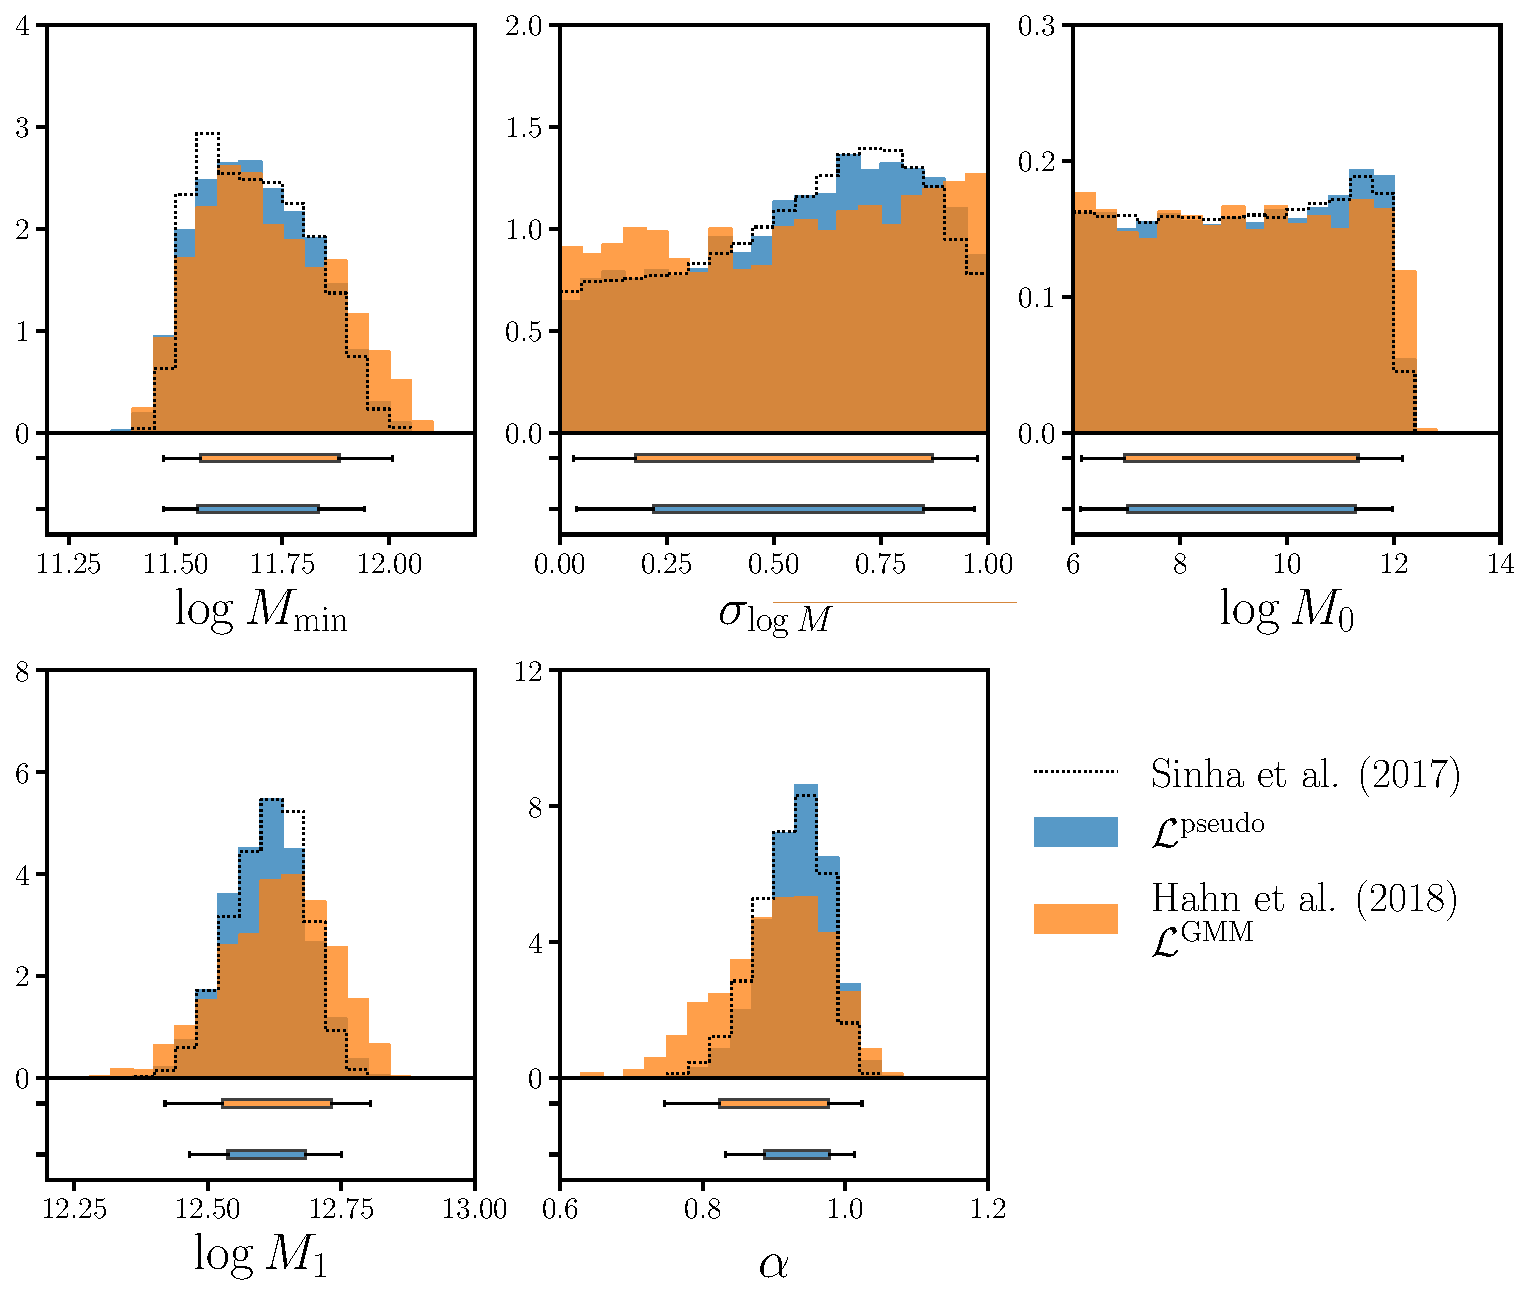
\includegraphics[width=0.9\textwidth]{figs/Like_GMF_comparison.pdf}
\caption{The posterior distribution for HOD parameters 
    $\log\, M_\mathrm{min}$, $\sigma_{\log\,M}$, 
    $\log\, M_0$, $\log\, M_1$, and $\alpha$ in the~\Sinh~$\zeta$ 
    analysis using the non-Gaussian GMM likelihood (orange). We 
    include in blue the posteriors calculated from the pseudo-likelihood
    for comparison. We also include the original~\Sinh~posterior 
    (dotted; see text for details). On the bottom of each panel we 
    include box plots that mark the $68\%$ and $95\%$ confidence 
    intervals of the posterior. Besides the poorly constrained 
    parameters $\sigma_{\log M}$ and $\log\, M_0$, the posteriors of 
    $\log\,M_\mathrm{min}$, $\log M_1$, and $\alpha$, are significantly 
    broader and shifted compared to the pseudo-likelihood constraints. 
    Likelihood non-Gaussianity significantly impacts the parameter
    constraints of the $zeta$ analysis. Therefore using the pseudo-likelihood  
    underestimates the uncertainty and biases the HOD parameter constraints. 
    }
\label{fig:gmf_like}
\end{center}
\end{figure}
%%%%%%%%%%%%%%%%%%%%%%%%%%%%%%%%%%%%%

%%%%%%%%%%%%%%%%%%%%%%%%%%%%%%%%%%%%%
% Figure 8 
%%%%%%%%%%%%%%%%%%%%%%%%%%%%%%%%%%%%%
\begin{figure}
\begin{center}
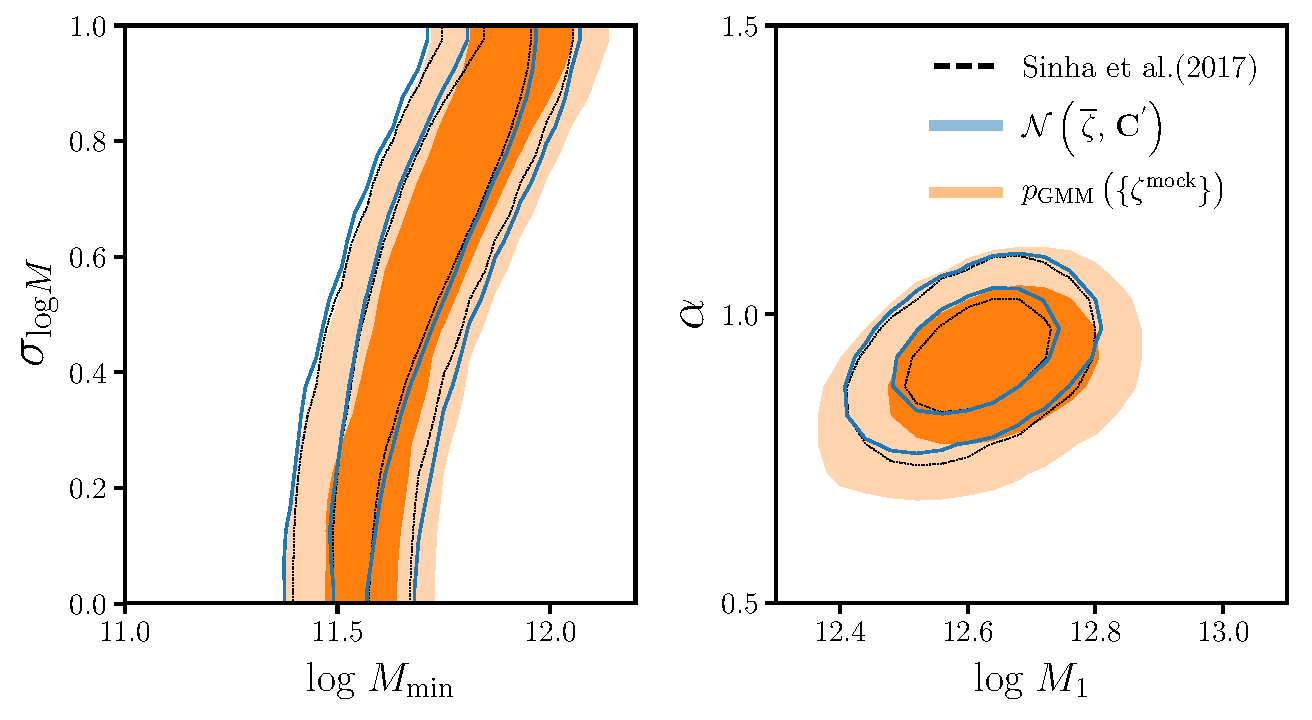
\includegraphics[width=0.8\textwidth]{figs/GMFcontours_manodeep.pdf}
\caption{Joint posterior distributions of select HOD parameters
    in the~\Sinh~$\zeta$ analysis, compute using the non-Gaussian 
    GMM likelihood (orange). We include, in blue, the posteriors 
    computed using the pseudo-likelihood; we also include the 
    original~\Sinh~posterior (dotted; see text for details). 
    The contours confirm that that \emph{due to likelihood 
    non-Gaussianity, posteriors from the pseudo-likelihood underestimate 
    the uncertainties and significantly biases the parameter constraints 
    of the \Sinh~analysis.} 
    }
\label{fig:gmf_contour}
\end{center}
\end{figure}
%%%%%%%%%%%%%%%%%%%%%%%%%%%%%%%%%%%%%

%%%%%%%%%%%%%%%%%%%%%%%%%%%%%%%%%%%%%
% Table 1 
%%%%%%%%%%%%%%%%%%%%%%%%%%%%%%%%%%%%%
\begin{table}
\caption{Impact of likelihood non-Gaussianity on the posterior parameter constraints of \Beut~and~\Sinh}
\begin{center}
\begin{tabular}{cccccccc} \toprule
    \multicolumn{8}{c}{\Beut~$P_\ell$ analysis} \\%[-7pt]
    \multicolumn{1}{c}{} & 
    \multicolumn{1}{c}{$f \sigma_8$} & 
    \multicolumn{1}{c}{$\alpha_\parallel$} & 
    \multicolumn{1}{c}{$\alpha_\perp$} & 
    \multicolumn{1}{c}{$b_1^\mathrm{NGC} \sigma_8$} & 
    \multicolumn{1}{c}{$b_1^\mathrm{SGC} \sigma_8$} &
    \multicolumn{1}{c}{$b_2^\mathrm{NGC} \sigma_8$} & 
    \multicolumn{1}{c}{$b_2^\mathrm{SGC} \sigma_8$} \\
    \hline
    \multicolumn{1}{c}{\Beut} & 
    \multicolumn{1}{c}{0.478} & 
    \multicolumn{1}{c}{$\alpha_\parallel$} & 
    \multicolumn{1}{c}{$\alpha_\perp$} & 
    \multicolumn{1}{c}{$b_1^\mathrm{NGC} \sigma_8$} & 
    \multicolumn{1}{c}{$b_1^\mathrm{SGC} \sigma_8$} &
    \multicolumn{1}{c}{$b_2^\mathrm{NGC} \sigma_8$} & 
    \multicolumn{1}{c}{$b_2^\mathrm{SGC} \sigma_8$} \\ 
    \multicolumn{1}{c}{\specialcell{non-Gaussian\\ $\mathcal{L}_\mathrm{ICA}$}} &  
    \multicolumn{1}{c}{0.478} & 
    \multicolumn{1}{c}{$\alpha_\parallel$} & 
    \multicolumn{1}{c}{$\alpha_\perp$} & 
    \multicolumn{1}{c}{$b_1^\mathrm{NGC} \sigma_8$} & 
    \multicolumn{1}{c}{$b_1^\mathrm{SGC} \sigma_8$} &
    \multicolumn{1}{c}{$b_2^\mathrm{NGC} \sigma_8$} & 
    \multicolumn{1}{c}{$b_2^\mathrm{SGC} \sigma_8$} \\[10pt]
    \hline 
    \hline
    \multicolumn{8}{c}{\Sinh~$\zeta$ analysis} \\%[-7pt]
\hline
\end{tabular} \label{tab:posterior} 
\end{center}
\end{table}
%%%%%%%%%%%%%%%%%%%%%%%%%%%%%%%%%%%%%


\section{Summary and Discussion} \label{sec:summary}
Standard present day LSS analyses makes a major assumption in their 
parameter inference --- the likelihood has a Gaussian functional-form. 
Although this assumption is motivated by the Central Limit Theorem, 
in detail this assumption cannot be true. 
In this paper, we investigate the impact of this assumption on two recent 
LSS analyses: the \Beut~powerspectrum multipole ($\ell = 0, 2$, and $4$) 
analysis and the \Sinh~group multiplicity function analysis. We combine 
mock catalogs, originally constructed 
for covariance matrix estimation in these analyses, with non-parametric 
divergence estimators to measure the divergences between the $P_\ell$ and 
$\zeta$ likelihoods and the Gaussian pseudo-likelihoods from \Beut~and~\Sinh. 
For both the $P_\ell$ and $\zeta$ likelihoods, the divergences reveal 
significant likelihood non-Gaussianity. \todo{More details on how 
the $\zeta$ likelihood is more non-Gaussian than the $P_\ell$ 
likelihood}

From the same mock catalogs of~\Beut~and~\Sinh, we use non-parametric density 
estimation to construct estimates of the likelihood distribution 
that better approximates the true non-Gaussian $P_\ell$ and $\zeta$ 
likelihoods. For the $\zeta$ likelihood, the direct method 
of estimating the likelihood distribution with the mocks and Gaussian
mixture density estimation results in an accurate estimate. For the 
\Beut~$P_\ell$ analysis, which has fewer mocks and a higher dimensional 
likelihood, we use Independent Component Analysis to transform the 
likelihood distribution into statistically independent components. 
By estimating the one-dimensional distribution of these independent 
components, we derive an estimate of the high-dimensional likelihood 
distribution. The divergence between these two likelihood estimates and 
the $P_\ell$ and $\zeta$ likelihoods demonstrate that we derive 
\emph{more accurate} estimates of the true likelihoods than the 
pseudo-likelihoods. 

Finally, using the $P_\ell$ and $\zeta$ likelihood estimates and importance 
sampling, we derive posterior parameter constraint for the \Beut~and~\Sinh 
analyses. Since our likelihood estimates are closer to the true likelihood, 
they allow us to derive more accurate posterior probability distributions 
than with Gaussian pseudo-likelihoods. By comparing our posteriors to the
parameter constraints from \Beut~and~\Sinh, we find that likelihood 
non-Gaussianity does not significantly impact the $P_\ell$ analysis of \Beut. 
Among the non-nuissance parameters, only $f\sigma_8$ is impacted by \todo{number}. 
Meanwhile for the \Sinh~$\zeta$ analysis, likelihood non-Gaussianity 
significant impacts the posterior distributions of the HOD parameter. 
Using the pseudo-likelihood significantly underestimates the width of the 
$\log\,M_\mathrm{min}$, $\log\, M_1$, and $\alpha$ posteriors. It also 
significantly biases their constraints. In fact, accounting for likelihood 
non-Gaussianity, significantly eases the tension between the $\zeta$ and 
$w_p(r_p)$ constraints found in \Sinh. Our comparisons of the posteriors 
ultimately highlight the significance of likelihood non-Gaussianity in 
parameter inference of LSS studies. 

Based on our results, $P_\ell$ analyses using future surveys (\emph{e.g.} 
DESI) will not be significantly impacted by likelihood non-Gaussianity.
While these analyses seek to extend the $k$ ranges probed, future surveys
will also expand the cosmic volumes probed by galaxies and increase the 
number of modes on all scales. We therefore expect Central Limit Theorem 
to reduce the impact of likelihood non-Gaussianity. Likewise, we expect
future surveys to also reduce the impact of likelihood non-Gaussianity on 
$\zeta$ analysis with the same multiplicity range, since larger cosmic 
volumes will probe more high multiplicity groups. For a wider multiplicity 
range, however, likelihood non-Gaussianity may still be a 
significant effect. For higher order statistics such as the galaxy bispectrum 
or three-point function, even for future surveys, likelihood non-Gaussianity 
may still be a significant effect to consider for parameter inference.  
Regardless of our expectation, for ever more precise parameter inference the Gaussian 
likelihood assumption must be extensively tested. The divergence and likelihood 
estimations we introduce in this paper provide a straightforward framework
for testing and quantifying the impact of likelihood non-Gaussianity on 
the final parameter constraints. 

Our likelihood estimation methods allow us to go beyond the pseudo-likelihood 
and derive more accurate estimates of the likelihood. With a similar 
motivation at addressing likelihoods that are non-Gaussian or difficult to 
write down, methods for likelihood-free inference such as Approximate Bayesian 
Computation~\citep[ABC;][]{hahn2017a,kacprzak2017,alsing2017} have recently 
been introduced to LSS studies. 
Although as a likelihood-free inference method, ABC has the advantage 
of relaxing any assumption on the likelihood, even with smart sampling methods 
like Population Monte Carlo, it requires an expensive generative forward 
model to be computed far more times than the number of mocks required for 
covariance matrix estimation. Our methods (especially the ICA method)
do not require any more mocks than those already constructed for accurate covariance 
matrix estimation. Therefore, the methods for likelihood estimation we present
in this paper provide both accurate and practical methods for Bayesian 
parameter inference in LSS. 

%%%%%%%%%%%%%%%%%%%%%%%%%%%%%%%%%%%%%%%%%%%%%%%%%%%%%%%%%%%%%%%
% Acknowledgements
%%%%%%%%%%%%%%%%%%%%%%%%%%%%%%%%%%%%%%%%%%%%%%%%%%%%%%%%%%%%%%%
\section*{Acknowledgements}
It's a pleasure to thank 
    Simone~Ferraro,
    David~W.~Hogg,
    Emmaneul~Schaan, 
    Uro{\u s}~Seljak,
    and Roman~Scoccimarro 
for valuable discussions.
\todo{more acknowledgements}
This project made use of the NASA Astrophysics Data System
and open-source software Python, numpy, SciPy, matplotlib, 
and Scikit-learn.

\bibliographystyle{yahapj}
\bibliography{nongausslike}
\end{document}
